\documentclass{article}
\usepackage[utf8]{inputenc}
\usepackage{indentfirst}
\usepackage{titling}
\usepackage{geometry}
\usepackage{graphicx}
\usepackage[shortlabels]{enumitem}
\usepackage{fancyhdr}
\usepackage{ulem}
\renewcommand\maketitlehooka{\null\mbox{}\vfill} %para centralizar verticalmente
\renewcommand\maketitlehookd{\vfill\null}
\pagestyle{fancy}
\fancyhf{}
\rfoot{\thepage}
\lfoot{ 
\includegraphics[scale=0.01]{UA.jpg} José Mendes 107188 LEI}
\geometry{
  a4paper,
  headheight=4cm,
  top=5.5cm,
  bottom=4.5cm,
  footskip=4cm
}


\title{Padrões e Desenho de Software}
\author{José Mendes 107188}
\date{2023}

\begin{document}


\begin{titlepage}
    \maketitle
    \begin{center}
        
\includegraphics[scale=0.4]{UA.png}
    \end{center}
    \thispagestyle{empty} %remove o count da pagina
\end{titlepage}

\pagebreak
%depois por um index aqui

\section{Introdução ao Desenho de Software}

\subsection{Desenho é uma atividade universal}

\par
Qualquer produto que é um agregado de elemento mais simples,
pode beneficiar da atividade que é o Desenho (Design).

\subsection{O que é o Desenho de Software?}

\par
No Software, este Desenho começa pela definição de \textbf{requisitos}.
Este processo deve ser efetuado pelo programador junto dos Stakeholders,
pelo que é fundamental este ter uma boa capacidade de comunicação e filtragem,
devendo durante o mesmo ficar escalrecidas quais as \uline{necessidades
do sistema a implementar}.

\vspace{2mm}
\par
A seguinte fase é o \textbf{desenho}, onde se \uline{definem as classes,
os métodos, as relações entre elas, os fluxos de trabalho, etc.}

\vspace{2mm}
\par
Todo o processo finda na \textbf{contrução}, que segue os dois processos
anteriores e já consiste na \uline{escrita de código que implemente
o sistema delineado}.

\vspace{2mm}
\par
É importante que durante estes procedimentos sejam considerados diferentes
níveis de detalhe do sistema:

\begin{enumerate}
    \item Sistema
    \item Subsistemas/pacotes: User Interface, Data Storage, Application-level Classes, Graphic\dots
    \item Classes dentro de pacotes, Relações entre classes, A Interface de cada Classe, métodos públicos 
    \item Atributos, Métodos privados, "Inner classes"\dots
    \item Código fonte que implementa os métodos
\end{enumerate}

\subsection{O Desenho ocorre em diferentes níveis}
\vspace{2mm}
\begin{center}
    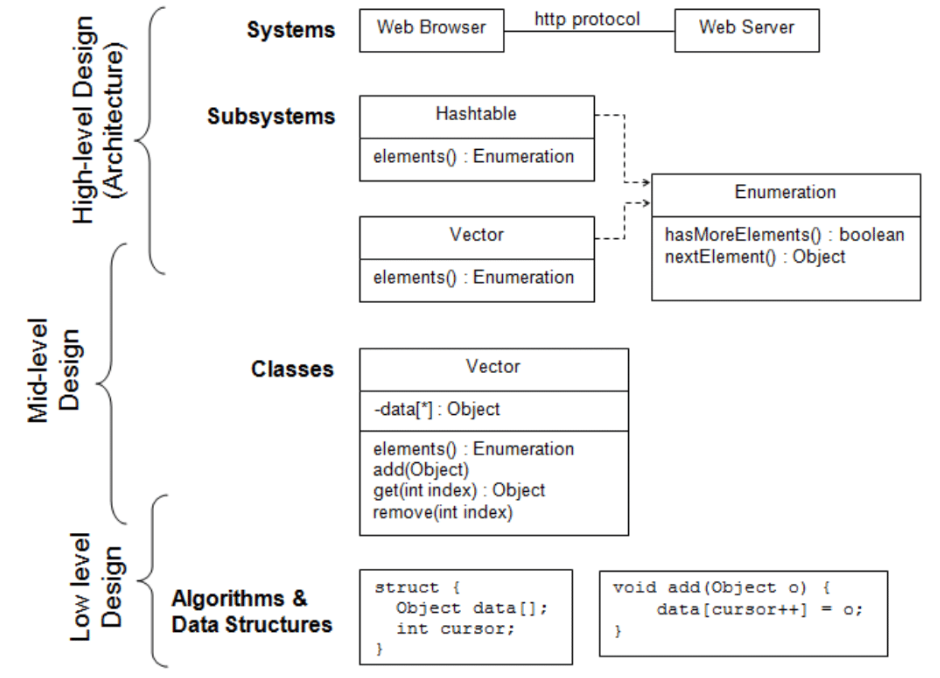
\includegraphics[scale=0.3]{Images/1.png}
\end{center}

\subsection{A importância do Desenho de Software}

\par
O processo de Desenho pode ser tornado mais \textbf{sistemático} e \textbf{previsível}
através da aplicação de métodos, técnicas e padrões, todos aplicados de acordo com
princípios e heurísticas.

\begin{center}
    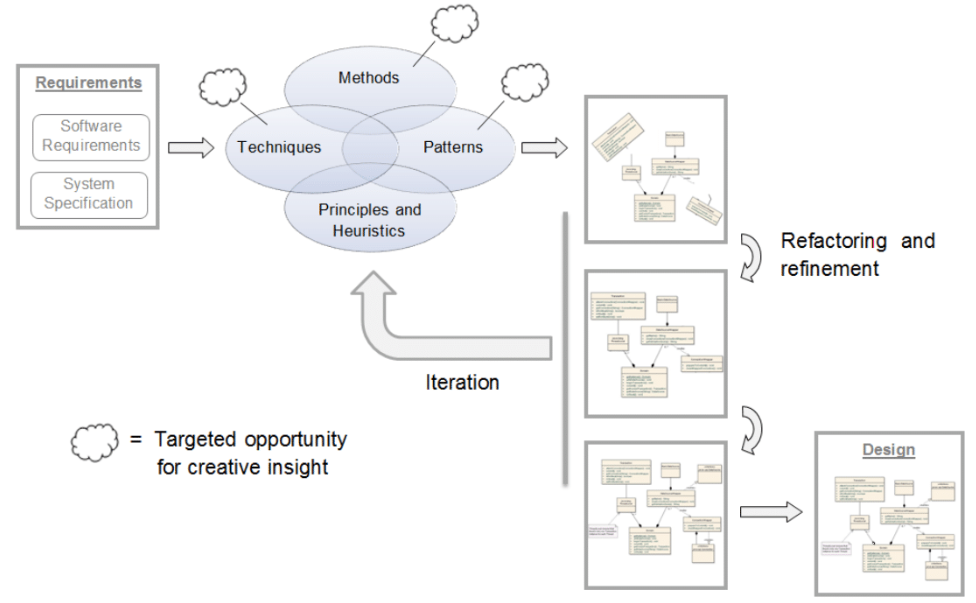
\includegraphics[scale=0.4]{Images/2.png}
\end{center}

\pagebreak

\subsection{A importância de controlar a complexidade}

\par
Um programa que seja mal desenhado, ou seja, muito complexo, é \uline{difícil de entender
e modificar}, podendo, a curto prazo, se mais rápido de desenvolver, mas acabando por
se tornar \uline{insustentável a longo prazo}.

Quanto maior for o programa, mais pronunciadas são as consequências de um mau desenho.

\begin{center}
    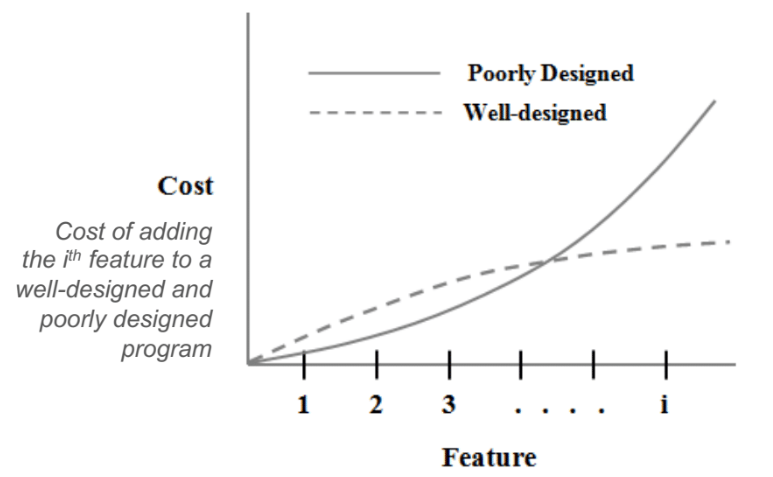
\includegraphics[scale=0.3]{Images/3.png}
\end{center}

\subsection{Dois tipos de complexidade no Software}

\par
O desenho é, portanto, uma ferramenta poderosa para o \textbf{controlo da complexidade}
no desenvolvimento de Software, gerindo:

\begin{flushleft}
    \textbf{Complexidades Essenciais -} São herdadas no problema

    \textbf{Complexidades Acidentais -} Associadas à solução e à forma como é implementada
\end{flushleft}

\par
A quantidade total de complexidade numa solução de Software é:

\begin{center}
    $Complexidades Essenciais + Complexidades Acidentais$
\end{center}

O objetivo é portanto, \textbf{controlar as Complexidades Essenciais, enquanto impedimos
a introdução de Complexidades Acidentais adicionais}.

\subsection{Lidar com Complexidade de Software}

Para evitar a complexidade no Desenho de Software devemos ter em conta os seguintes
princípios:

\begin{flushleft}
    \textbf{Modularidade -} \uline{Subdividir} a solução em componentes mais pequenos e fáceis
    de controlar (DaC - Divide and Conquer).

    \textbf{Abstração -} Usar abstração para \uline{omitir detalhes} em sítios que estes não são
    necesários

    \textbf{Esconder Informação -} Esconder detalhes e complexid\uline{}ades através de \uline{interfaces
    simples}

    \textbf{Herança -} \uline{Componentes genéricos} podem ser \uline{reutilizados} para definir
    elementos mais específicos

    \textbf{Composição -} \uline{Reutilizar outros componentes} para contruir uma nova \uline{solução}
\end{flushleft}

\pagebreak

\subsection{O Desenho é um "Wicked Problem"}

Um "Wicked Problem" é um problema que apenas pode ser definido claramente, através de uma solução.

\begin{flushright}
    "TEX would have been a complete failure if I had merely specified it
    and not participated fully in its initial implementation.
    The process of implementation constantly led me to unanticipated questions
    and to new insights about how the original specifications could be improved."

    \vspace{2mm}

    -Donald Knuth
\end{flushright}

\subsection{Características do Desenho de Software}

O desenho de Software caracteriza-se por ser:

\begin{flushleft}
    \textbf{Não determinístico -} Uma vez que a maioria dos processos de desenho
    para o mesmo programa não atingem o mesmo resultado (output diferente)

    \textbf{Heurístico -} Uma vez que as técnicas de desenho apoiam-se em heurísticas e
    em regras práticas (rules-of-thumb) em vez de processos repetitivos

    \textbf{Emergente -} Uma vez que o resultado final evolui de acordo com a
    experiência e o feedback. O desenho é um processo iterativo e incremental onde
    a complexidade do sistema surge de interações relativamente simples
\end{flushleft}

Desta forma, é fundamental acompanhar todas as fases de desenvolvimento, pois elas
estão fortemente interligadas e durante o desenvolvimento de uma pode haver necessidade
de reaçizar alterações nas anteriores.

Com este trabalho é \uline{criado um sistema complexo, como resultado de pequenas e
simples iterações}.

\subsection{Processo de Desenho Genérico}

\begin{enumerate}
    \item \textbf{Perceber} o problema (definição de requisitos de Software);
    \item Contruido um \textbf{modelo de solução}, "black-box", sendo as especificações
    de sistema geralmente representadas por \uline{casos de uso (use cases)};
    \item \textbf{Procurar por soluções existentes}, como por exemplo padrões de arquitetura ou desenho
    que abrangem alguns/todos os problemas identificados pelo desenho de Software;
    \item Considerar contruir \textbf{protótipos};
    \item Documentação e \textbf{revisão} do desenho;
    \item \textbf{Refactor} (Iterate over the solution), ou seja, evoluir o desenho até
    ter os requisitos funcionais e maximixar os requuisitos não funcionais;
\end{enumerate}

\pagebreak

\subsection{Entradas (Inputs) para o processo de desenho}

\begin{enumerate}
    \item \textbf{Requisitos do utilizador} e especificações de sistema, incluindo qualquer restrição no desenho e implementação de opções;
    \item \textbf{Conhecimento do domínio}, por exemplo, se for uma aplicação de um centro de saúde, o designer necessita de algum conhecimento dos termos e conceitos destes centros;
    \item \textbf{implementação do conhecimento}, capacidades e limitações de eventuais ambientes de execução; 
\end{enumerate}

\subsection{Desenho de características interno desejado}

\begin{flushleft}
    \textbf{Complexidade mínima -} Manter simples. Talvez não seja preciso altos níveis de generalidade

    \textbf{Loose Coupling -} Minimizar dependências entre modelos

    \textbf{Manutenção fácil -} O teu código vai ser mais vezes lido do que escrito

    \textbf{Extensibilidade -} Desemho para hoje mas olhando para o futuro.
    \uline{Nota}: Esta característica pode estar em conflito com a primeira, complexidade mínima.
    Engenharia é balanciar objetivos em conflito

    \textbf{Reutilizavél -} Reutilização é um sinal da maturidade da Engenharia

    \textbf{Portável -} Funciona ou pode facilmente funcionar em outros ambientes

    \textbf{Fan-in alto -} Em alguns módulos utility-type e low-to-medium fan-out em todos os módulos.
    Fan-out elevado está tipicamente associado a complexidade elevada

    \textbf{Magreza -} Quando em dúvida, deixar de fora. O custo de adicionar outra linha de
    código é muito mais do que os poucos minutos necessários para a escrever

    \textbf{Estratificação -} Em camadas. Mesmo se todo o sistema não seguir a arquitetura
    por camadas, componentes individuais podem fazê-lo

    \textbf{Tecnicas base -} Por vezes é bom ser um conformista! Ser secante é bom.
    Código de produção não é o local para tentar experimentar técnicas
\end{flushleft}

\vspace{3mm}

\begin{center}
    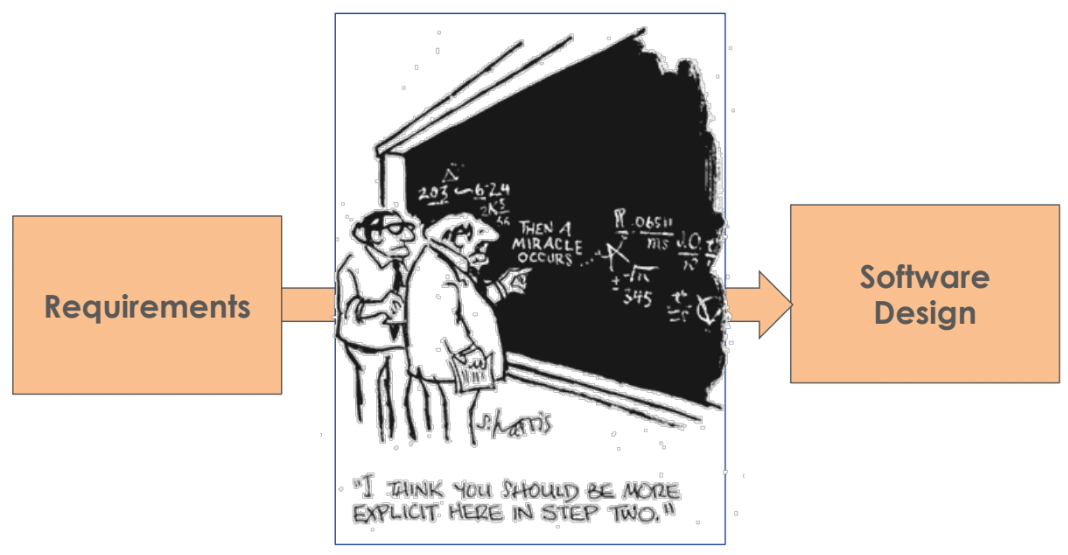
\includegraphics[scale=0.3]{Images/4.png}
\end{center}

\pagebreak

\subsection{Padrões}

\begin{flushleft}
    \textbf{Padrão de Desenho-} Solução para um problema de desenho comum reutilizável
\end{flushleft}

Os padrões de desenho são adaptados às características do problema que resolvem e dependendo
do nível de desenho a que se aplicam, os padrões de desenho podem ser divididos em \textbf{padrões arquiteturais,
padrões de desenho ou idiomas de programação}.

\vspace{3mm}
Não existe uma metodologia melhor para obter o melhor desenho de orientado a objetos,
no entanto existem princípios, padrões, heurísticas.

\vspace{3mm}

\begin{center}
    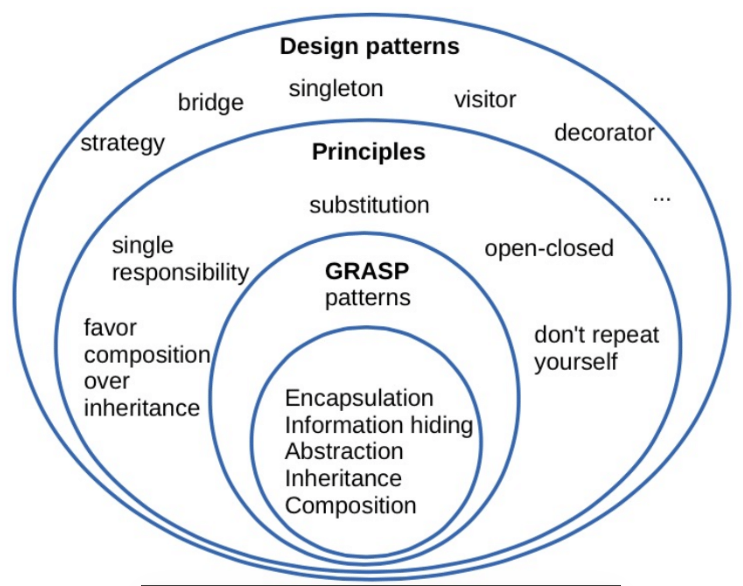
\includegraphics[scale=0.4]{Images/5.png}
\end{center}

\pagebreak
% segundo ppt
\subsection{Os diferentes modelos e a sua representação}

Em diferentes fases do desenho de Software são utilizados diferentes modelos para a
sua representação. O \textbf{domínio de modelo} representa um modelo conceptual,
incorporando tanto o comportamento, como a informação de cada entidade.

\begin{center}
    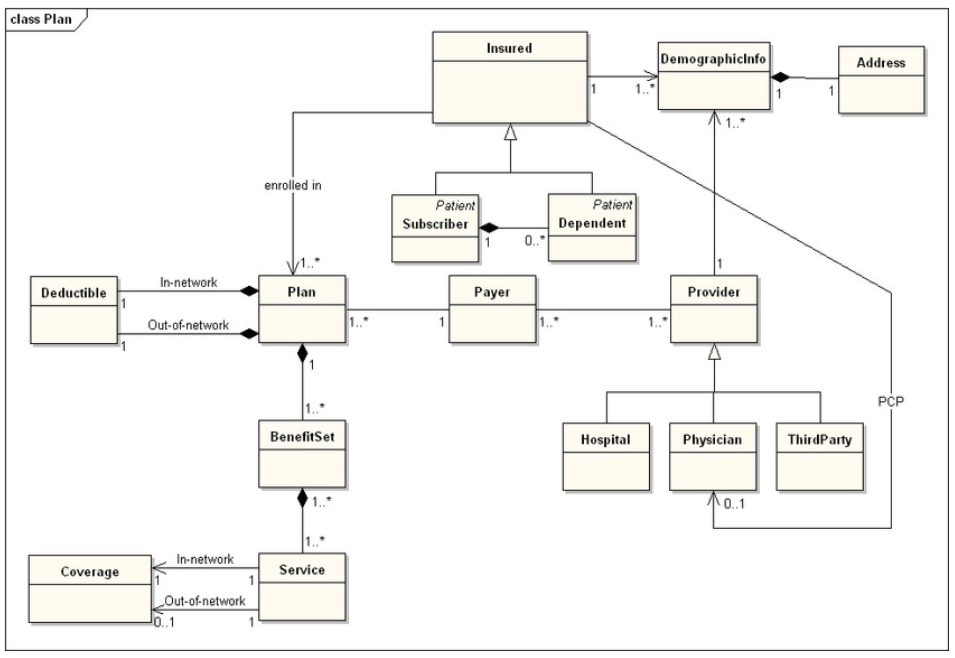
\includegraphics[scale=0.3]{Images/6.png}
\end{center}

Nestes, a herança e a composição são respetivamente representados por:

\begin{center}
    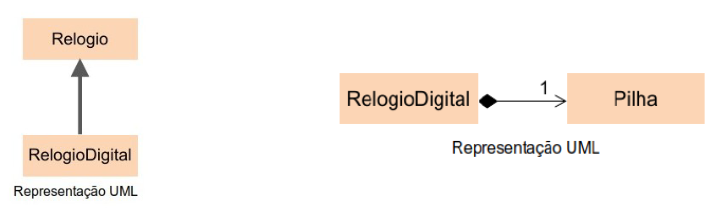
\includegraphics[scale=0.4]{Images/7.png}
\end{center}

É também muito comum a utilização do domínio dinâmico, este mais focado na
evolução temporal dos objetos.

\begin{center}
    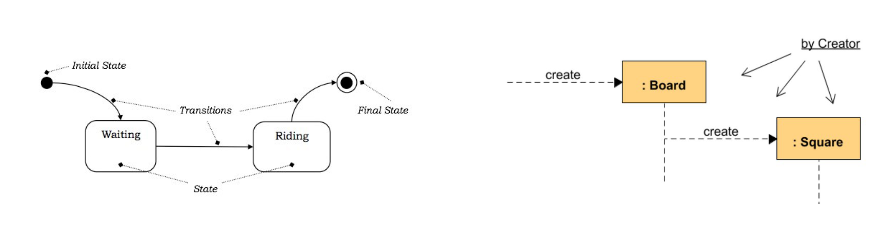
\includegraphics[scale=0.4]{Images/8.png}
\end{center}    


\pagebreak

Para modelar as interações num comportamento gerado num caso de uso particular
utilizam-se diagramas de colaboração.

\begin{center}
    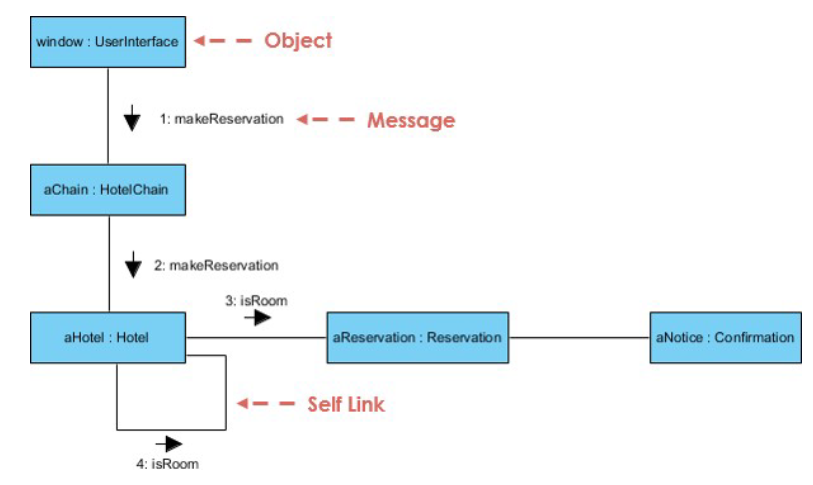
\includegraphics[scale=0.4]{Images/9.png}
\end{center}

\section{Princípios GRASP}

Uma das metodologias de desenvolvimento de Software mais comuns designa-se
\textbf{Responsability-driven Design, RDD} e consiste na definição dos objetos
em termos de \uline{responsabilidade, papeis e colaboração}.

\begin{flushleft}
    \textbf{Nota:} As responsabilidades podem ser generalizadas em \textbf{fazer}, seja criar um objeto, fazer um cálculo,
    despoletar ações ou coordenar atividades noutros objetos e \textbf{saber}, por exemplo, os seus dados privados,
    objetos relacionados, etc.
\end{flushleft}

Estas por sua vez são implementadas através de \textbf{métodos}, que podem atuar
sozinhos ou em colaboração com outros.

Os  \textbf{General Responsability Assignment Software Patterns, GRASP} são uma
resposta à criação desta metodologia, \uline{descrevendo os princípios fundamentais do desenho
e atribuição de responsabilidade aos objetos}.

\begin{flushleft}
    \textbf{Nota:} A tradução literal de grasp é compreender, sendo esta analogia propositada para destacar a importância
    do domínio dos princípios fundamentais para ter sucesso no desenvolvimento de software.
\end{flushleft}


\pagebreak

De uma forma geral:

\begin{enumerate}
    \item Atribuir responsabilidade a uma classe
    \item Evitar ou Minimizar dependências adicionais
    \item Maximizar a coesão (cohesion) e Minimizar o acoplamento (coupling)
    \item Aumentar a reutilização e reduzir a manutenção
    \item Maximizar a compreensão do código\dots
\end{enumerate}

\begin{flushleft}
    \textbf{Nota:} A maioria dos padrões definidos pelos GRASP são conhecimento comum. No entanto, há a necessidade de
    os estandardizar, dando-lhes um nome e registando o seu funcionamento, facilitando assim a
    comunicação entre programadores e a memorização por parte dos mesmos.
\end{flushleft}

Os princípios GRASP são:

\begin{enumerate}
    \item Creator
    \item Information Expert
    \item Low Coupling
    \item High Cohesion
    \item Controller
    \item Polymorphism
    \item Pure Fabrication
    \item Indirection
    \item Protected Variations
\end{enumerate}

\pagebreak

\subsection{Creator}

\begin{flushleft}
    \textbf{Nota:} Como resposta, a maioria dos programadores pensa imediatamente no container criar o elemento contido.
    Este raciocínio tem por base o \textbf{low representational gap} e não está errado.

    Na verdade, existem mais alguns critérios, sendo as condições para B criar A listadas abaixo.
\end{flushleft}

\begin{flushleft}
    \textbf{Problema:} Quem cria a instância de A? (Fazer)

    \vspace{3mm}
    \textbf{Solução:} Atribuir à classe B a responsabilidade de criar uma instância
    da classe A se uma destas for verdade (quantas mais melhor):

    \begin{enumerate}
        \item B \textbf{contém} ou \textbf{agrega} (contem um conjunto de) A;
        \item B \textbf{regista} A;
        \item B \textbf{utiliza} com frequência A;
        \item B \textbf{tem os dados de inicialização} de A;
    \end{enumerate}
\end{flushleft}

\begin{flushleft}
    \textbf{Exemplo:}

    \vspace{3mm}
    Num jogo de monopólio e segundo este princípio, o \uline{tabuleiro cria as casas}, uma vez que um tabuleiro
    agrega (tem uma coleção) de casas.

    \begin{center}
        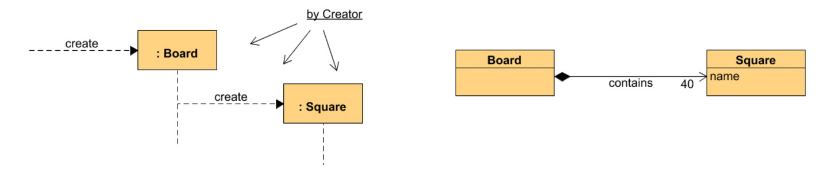
\includegraphics[scale=0.5]{Images/10.png}
    \end{center}

    \vspace{3mm}
    Num POS (Point of Sale), uma LinhaDeVenda é criada pela Venda, uma vez que a venda agrega várias
    linhas.

    \begin{center}
        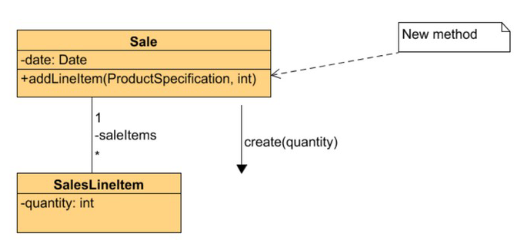
\includegraphics[scale=0.4]{Images/11.png}
    \end{center}
\end{flushleft}

Promove a minimização do acoplamento ao fazer uma instância de uma classe responsável
por criar os objetos que referenciam. (\textbf{Pró})

\pagebreak

Conectar um objeto ao seu Creator quando:

\begin{enumerate}
    \item Aggregator aggregates Part
    \item Container contains Content
    \item Recorder records
    \item Initializing data passed in during creation
\end{enumerate}

Pode levar ao aumento da complexidade, aquando da reciclagem de instâncias para
aumentar a performance e da criação condicional de instâncias através de uma
família de classes semelhantes. Nestes casos, aplicam-se outros princípios. (\textbf{Contra})

\subsection{Information Expert}

\begin{flushleft}
    \textbf{Problema:} Qual o princípio para atribuir responsabilidades a objetos? (Saber e Fazer)

    \vspace{3mm}
    \textbf{Solução:} Atribuir a responsabilidade à classe que tem a informação necessária para
    a assumir.

    \vspace{3mm}
    Este método baseia-se na filosofia de "Não faças nada que podes atribuir a outra
pessoa”.
\end{flushleft}

\begin{flushleft}
    \textbf{Exemplo:} No monopólio, a questão que está na origem deste princípio pode colocar-se na forma de \textbf{Quem tem o
    conhecimento das casas, dada uma chave?} Como vimos pelo princípio Creator, o tabuleiro vai criar as
    casas, sendo esta a classe que as agrega e por isso que tem informação sobre elas. Conclui-se assim que
    o \textbf{tabuleiro} é a classe indicada para \uline{assumir a responsabilidade de identificar} uma \textbf{casa} dada uma chave.

    \begin{center}
        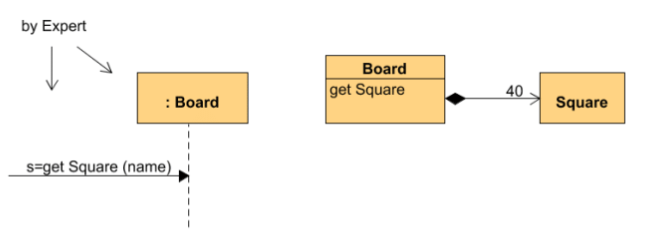
\includegraphics[scale=0.4]{Images/12.png}
    \end{center}

    \pagebreak
    No POS, o responsável por saber o total de uma venda será a classe Venda, uma vez que é ela que
    instancia as LinhasDeVenda, tendo por isso a informação necessária para assumir esta responsabilidade.
    Por sua vez, para calcular o total, a Venda necessita de saber o subtotal de cada linha, sendo para esta
    responsabilidade, a classe LinhaDeVenda a expert para assumir, uma vez que tem a referência do
    produto (onde acede ao preço unitário) e a sua quantidade. Por sua vez, para saber o seu preço, cada
    produto é o expert.

    \begin{center}
        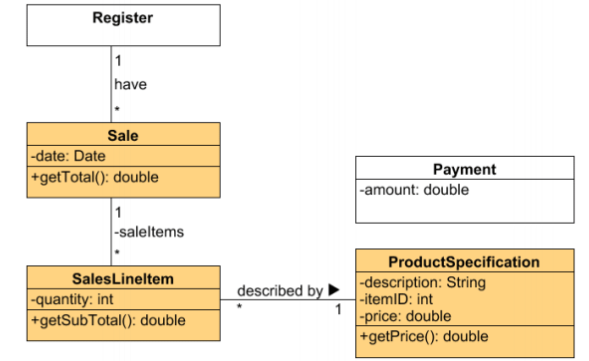
\includegraphics[scale=0.4]{Images/13.png}
    \end{center}

    A questão da complexidade levanta-se na dúvida de quem tem a responsabilidade de guardar a Venda na
    base de dados, sendo esta a classe expert, pois com a organização estipulada acima, cada classe
    apresenta os seus próprios serviços para se guardar na base de dados.
\end{flushleft}

\begin{flushleft}
    \textbf{Beneficios:} 
    
    - Facilita o encapsulamento de informação:
    \begin{enumerate}
        \item Cada classe utiliza assim a informação que dispõe para cumprir tarefas, tornando-se
        mais coesas
        \item Escrever código mais fácil de modo a ser percebido apenas lendo-o
    \end{enumerate}

    - Promove \textbf{low coupling}
\end{flushleft}

\begin{flushleft}
    \textbf{Contraindicações:}

    - Pode tornar uma classe excessivamente complexa, o que necessita outro tipo de separação, domínio e persistência.
\end{flushleft}

\pagebreak

\subsection{Low Coupling}

\begin{flushleft}
    \textbf{Problema:} Como reduzir o impacto da mudança e encorajar a reutilização?

    \vspace{3mm}
    \textbf{Solução:} Atribuir responsabilidades de forma a que o acoplamento se mantenha
    reduzido, tentando que uma classe conheça o menor número de outras.

    \vspace{3mm}
    \textbf{Nota:} O \textbf{acoplamento} define-se como o quão ligado, informado ou dependente está um elemento de outro.
    
    Uma classe X acopla a Y outra quando tem um \textbf{atributo} para uma instância da Y, quando um dos seus
    métodos instancia a Y, quando X é uma \textbf{subclasse} de Y ou Y é uma \textbf{interface} implementada por X.
\end{flushleft}

\begin{flushleft}
    \textbf{Exemplo:} No monopólio não faz sentido atribuir a responsabilidade de obter uma \textbf{casa} a uma classe \textbf{cão}, quando
    este teria de consultar o \textbf{tabuleiro}, a entidade expert sobre as casas.

    \begin{center}
        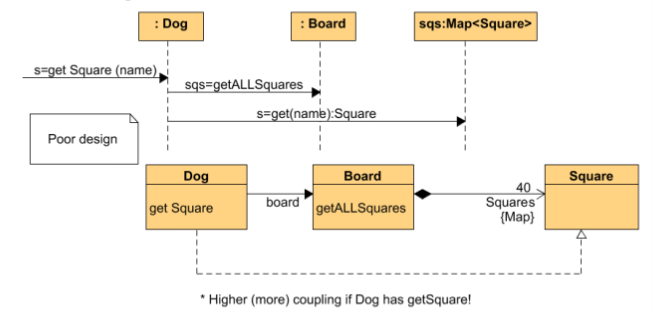
\includegraphics[scale=0.5]{Images/14.png}
    \end{center}

    Outro exemplo é a \textbf{peça}. Normalmente esta estaria associada a uma \textbf{casa}, que por sua vez está associada
    ao tabuleiro. Caso o tabuleiro tivesse informações da \textbf{peça} sem consultar a \textbf{casa}, seria estariamos
    perante um cenário de \uline{higher coupling} do que o anteriormente descrito.

    No POS, o método que cria um \textbf{Pagamento}, segundo este princípio deve estar na \textbf{Venda}, apesar de ser
    despoletado na sequência de outro método na \textbf{Venda} pela \textbf{CaixaRegistadora}.

    \begin{center}
        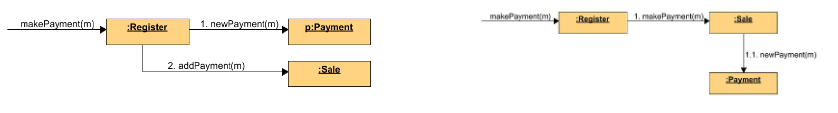
\includegraphics[scale=0.5]{Images/15.png}
    \end{center}
\end{flushleft}

\pagebreak

\begin{flushleft}
    \textbf{Beneficios:} 
    \begin{enumerate}
        \item Compreensão: Classes são mais fáceis de compreender quando isoladas
        \item Manter: Classes não são afetadas pelas mudanças em outros componentes
        \item Reutilizavél: Fácil de aceder a outras classes
    \end{enumerate}
\end{flushleft}

\begin{flushleft}
    \textbf{Contraindicações:} Em classes estáveis, um acoplamento maior não é um grande problema.
\end{flushleft}

\begin{flushleft}
    \textbf{Nota:} Os princípios do método Information Expert, visto anteriormente, servem de suporte a este princípio, pois
    procuramos a classe que tem mais informação para cumprir a responsabilidade.
\end{flushleft}

É impossível ter um acoplamento nulo, uma vez que é também fundamental que as
classes troquem mensagens entre si. Deve é ser na medida certa!

\subsection{High Cohesion}

\begin{flushleft}
    \textbf{Problema:} Como manter as classes focadas, percetíveis e maleáveis?

    \vspace{3mm}
    \textbf{Solução:} Atribuir responsabilidades de forma a manter uma alta coesão.
\end{flushleft}

A coesão diminui com o aumento da quantidade de código e da diversidade de
funcionalidades. O objetivo é então delegar responsabilidades e coordenar o
trabalho.
Geralmente uma baixa coesão está aliada a um elevado acoplamento.

\begin{flushleft}
    \textbf{Exemplo:} No monopólio, uma implementação em que a classe \textbf{Jogo} faça todas as tarefas é pouco coesa, sendo
    preferível uma em que esta delega noutras as várias tarefas, coordenando-las.

    \begin{center}
        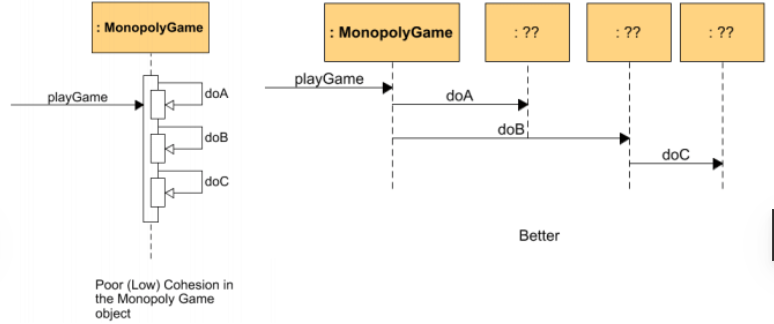
\includegraphics[scale=0.4]{Images/16.png}
    \end{center}

    No exemplo do POS dado no princípio do Low Coupling, o ideal também cumpre os princípios de alta
    coesão.
\end{flushleft}

\vspace{3mm}

\begin{flushleft}
    \textbf{Beneficios:} 
    Este princípio torna o código mais fácil de compreender, manter, complementando o
    baixo acoplamento.
\end{flushleft}

\begin{flushleft}
    \textbf{Contraindicações:} Por vezes é necessário criar objetos pouco coesos, nomeadamente nas
    comunicações e objetos remotos, em que é necessário criar uma única interface para
    várias operações.
\end{flushleft}

\pagebreak

\subsection{Controller}

\begin{flushleft}
    \textbf{Problema:} Quem deve ser responsável por eventos UI?

    \vspace{3mm}
    \textbf{Solução:} Se um programa recebe eventos de fontes externas além do seu GUI,
    adicionar uma classe que desassocia o evento, separando e fazendo a ponte entre as fontes
    do evento e os objetos que lidam com estes.
\end{flushleft}

Atribuir a responsabilidade de lidar com a mensagem do evento do sistema a uma classe
representando uma destas duas escolhas:

\begin{enumerate}
    \item Classe representativa do modelo de negócio em que se insere, denominada de
    \textbf{façade controller}
        \item Classe artificial, seguindo o método Pure Fabrication, denominada de \textbf{case
        controller}
\end{enumerate}

\begin{flushleft}
    \textbf{Nota:} Limita-se a encaminhar os eventos e o output dos métodos ativados por este.
\end{flushleft}

\begin{flushleft}
    \textbf{Exemplo:} Num monopílio com interface visual interativa, quando o utilizador pressionar o botão para iniciar um novo
    \textbf{Jogo}, este evento deve ser gerido por uma classe do tipo controller, e não diretamente pelo Jogo.

    \begin{center}
        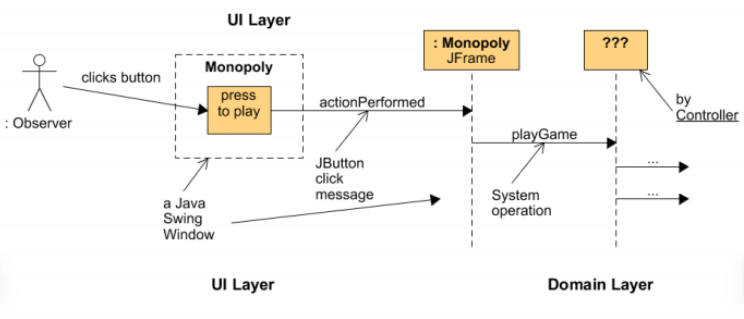
\includegraphics[scale=0.5]{Images/17.png}
    \end{center}
\end{flushleft}

\begin{flushleft}
    \textbf{Beneficios:} 
    Ao separar os eventos externos dos seus gestores internos, cria-se uma abstração
quanto ao tipo e comportamento das instâncias ligados pelo controller, que podem
ser modificadas sem interferir uma com a outra.

Permite-nos ainda garantir que as operações são realizadas numa sequência válida,
prevenindo assim a realização de ações ilegais que podem levar à criação de erros.
\end{flushleft}

\begin{flushleft}
    \textbf{Contraindicações:} Não tem
\end{flushleft}

\pagebreak
\subsection{Polymorphism}

\begin{flushleft}
    \textbf{Problema:} Como gerir o comportamento com base no tipo (i.e classe)
    mas sem usar os blocos if-then-else ou switch?

    \vspace{3mm}
    \textbf{Solução:} Quando comportamentos alternativos são selecionados com base
    no tipo do objeto, usar métodos polimórfimos para escolher o comportamento,
    em vez de usar instruções condicionais para testar o tipo.

    \uline{Métodos polimórfimos:} Atribuir o mesmo nome a serviços
    (métodos) distintos em classes diferentes. Os serviços são implementados por métodos.
\end{flushleft}

\begin{flushleft}
    \textbf{Exemplo:} Numa aplicação que lide com formas geométricas 2D, sabemos que existem formas diferentes cujo
    perímetro e área têm fórmulas distintas. Para evitar numa função que lide com todas a necesidade de
    determinar o seu tipo, podemos utilizar o polimorfimo.

    Fazemos assim com que todas as classes que representam uma forma geométrica implementem uma
    interface comum, que basicamente determina os métodos que estas vão implementar.

    \begin{center}
        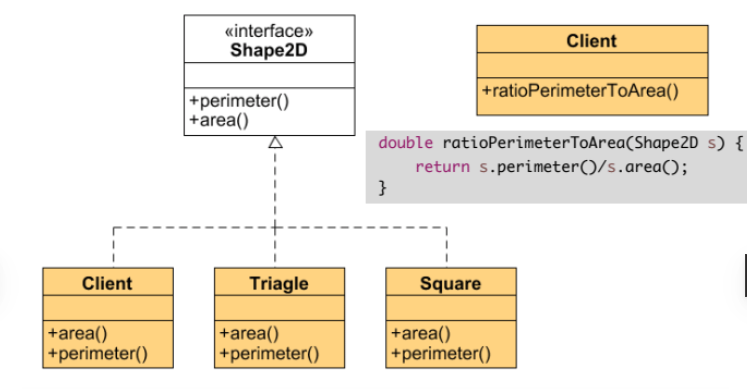
\includegraphics[scale=0.4]{Images/18.png}
    \end{center}
\end{flushleft}

\begin{flushleft}
    \textbf{Beneficios:} 
    Mais fácil e mais confiável do que usar lógica de seleção explicita.

    É mais fácil adicionar comportamentos mais tarde.

    Se o polimorfimo não for utilizado, e forem usados blocos condicionais,
    então, esta secção de código vai crescer à medida que mais tipos são adicionados
    ao sistema. A secção de código fica mais acopolada (sabe de mais tipos) e menos coesa
    (está a fazer demasiado).
\end{flushleft}

\begin{flushleft}
    \textbf{Contraindicações:} Não tem
\end{flushleft}

\pagebreak

\subsection{Pure Fabrication}

\begin{flushleft}
    \textbf{Problema:} Que objeto deve assumir uma resposabilidade quando nenhuma das classes
    do problema a pode assumir sem violar os princípios do low coupling e high
    cohesion?

    Esta pergunta coloca-se pois nem todas as responsabilidades se enquadram no domínio das classes, como
    por exemplo as comunicações, interação com o utilizador...

    \vspace{3mm}
    \textbf{Solução:} Atribuir um conjunto bastante coeso de responsabilidades a uma classe artificial que
    não representa nada no domínio no problema.
\end{flushleft}

\begin{flushleft}
    Por exemplo, no POS, se quisermos guardar o resgisto de cada venda numa base de dados relacional, pelo
    princípio Information Expert faria sentido atribui-la à classe \textbf{Venda}, no entanto, com esta atribuição a
    classe iria tornar-se pouco coesa e fortemente acoplada à base de dados.

    A solução que este princípio propõe é criar uma nova classe, responsável por guardar elementos na base
    de dados relacional, que vai ser invocada pela classe \textbf{Venda}.
    \begin{center}
        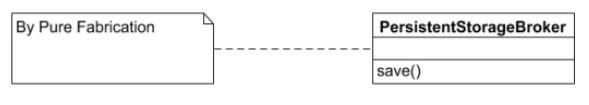
\includegraphics[scale=0.4]{Images/19.png}
    \end{center}

    Esta classe, por sua vez, pode ser fortemente reutilizada.

    Outro exemplo é numa classe Imagem, que segundo este princípio deve ser abstraída das operações de
    ser guardada em diferentes formatos.

    \begin{center}
        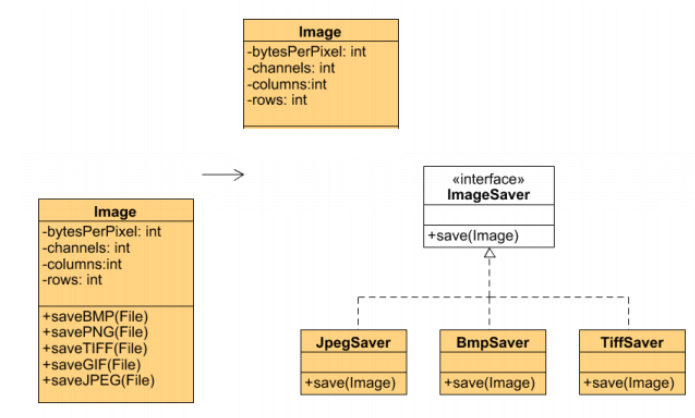
\includegraphics[scale=0.4]{Images/20.png}
    \end{center}
\end{flushleft}

\begin{flushleft}
    \textbf{Beneficios:} 
    Aliado ao princípio da alta coesão, uma vez que a classe artificial tem um foco muito
    específico.

    Potencial para a reutilização deve aumentar, devido à presença de várias classes.
    Pure Fabrication.
\end{flushleft}

\begin{flushleft}
    \textbf{Contraindicações:} Não tem
\end{flushleft}

\pagebreak

\subsection{Indirection}

\begin{flushleft}
    \textbf{Problema:} Como evitar acoplamento direto, desacoplando objetos de forma a
    suportar low coupling, e manter o potencial de reutilização elevado?
    \vspace{3mm}
    \textbf{Solução:} Atribuir a resposabilidade a um objeto intermédio. Para ser o mediador
    entre outros componentes e serviços, de forma a não ser diretamente acopolados.
\end{flushleft}

Indirection pode ser categorizada em:

\begin{enumerate}
    \item Behavioural Extension
    \item Interface Modification
    \item Technology Encapsulation
    \item Complexity Encapsulation
\end{enumerate}

\begin{flushleft}
    \textbf{Exemplo:} No princípio anterior, a criação de uma classe para gerir as interações com a base de dados é também um
    exemplo da aplicação deste método.

    Outro cenário em que este se aplica é no POS, nomeadamente devido à necessidade de estabelecimento
    de um canal de comunicação com um siste de pagamento para validar uma transação. Para tal, deve ser
    criada uma classe responsável por esta operação.
\end{flushleft}

\begin{flushleft}
    \textbf{Beneficios:} 
    Permite baixo acoplamento e promove a reutilização.
\end{flushleft}

\begin{flushleft}
    \textbf{Contraindicações:} Não tem
\end{flushleft}

\subsection{Protected Variations}

\begin{flushleft}
    \textbf{Problema:} Como desenhar software de forma a que as suas variações não tenham um
    impacto negativo noutros elementos?


    \vspace{3mm}
    \textbf{Solução:} Identificar os pontos de instabilidade e atribuir responsabilidades de forma a
    criar uma interface estável em sua volta.

    \vspace{3mm}
    \uline{Serve de base a muitos padrões de desenho!}
\end{flushleft}

\subsubsection{LiskovSubstitution Principle (LSP)}

Princípio com base no protected variations, defende que sendo B uma subclasse de
A, os objetos de A devem poder ser substituídos por B sem alterar a normal execução
do programa, ou seja:

\begin{enumerate}
    \item B não deve remover métodos implementados em A;
    \item Cada método de B que reescreva um definido em A não deve alterar o seu
    comportamento esperado, ou seja, não deve surpreender cliente!
\end{enumerate}

\begin{flushleft}
    \textbf{Exemplo:} Voltando ao exemplo das figuras geométricas, do ponto de vista matemático, um quadrado é um
    retângulo com os lados todos iguais. No entanto, num programa, onde o cliente espera encontrar uma
    instância de um retângulo, se lhe apresentarmos um quadrado, não vamos dar ao cliente o que ele espera,
    uma vez que ele não pode manipular as dimensóes de forma a ter uma largura diferente do comprimento.

    Devemos então, por forma a garantir a estabilidade da sua utilização, eliminar esta relação entre o
    quadrado e o retângulo, tornando-los classes distintas.

    \begin{center}
        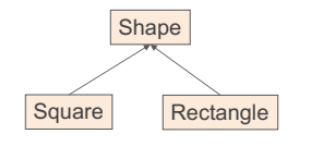
\includegraphics[scale=0.5]{Images/21.png}
    \end{center}
\end{flushleft}

\subsubsection{Law of Demeter (Don’t talk to strangers)}

Este é outro princípio que deriva do protected variations, estebelecendo que de
forma a evitar que objetos conheçam a estrutura de outros que não lhe estão
diretamente ligados, cada objeto só deve comunicar consigo, os seus parâmetros e
atributos, ou objetos criados pelos seus métodos.

\begin{flushleft}
    \textbf{Exemplo:} Numa Empresa dividida em Departamentos, cada um com um gestor, que é uma instância da classe
    Empregado, se a empresa quiser saber o total de dinheiro que paga aos gestores não deve invocar um
    método no Empegado, mas sim no Departamento, uma vez que este é seu atributo (o empregado
    não!).
\end{flushleft}

\begin{flushleft}
    \textbf{Beneficios:} 
    Mantém o coupling entre classes baixo e torna o desenho robusto

    Adiciona uma pequena quantidade de overhead no formato de métodos indiretos
\end{flushleft}

\begin{flushleft}
    \textbf{Contraindicações:} Não tem
\end{flushleft}

\subsection{Outros princípios}

\subsubsection{SOLID}

\vspace{3mm}
\begin{flushleft}
    \textbf{Single Responsability}
\end{flushleft}

Cada classe deve assumir uma única responsabilidade e ser encapsulada interiamente pela classe
(encapsulamento máximo).

\vspace{2mm}
\begin{flushleft}
    \textbf{Open/closed (OCP)}
\end{flushleft}

As entidades de Software devem estar abertas à extensão, mas fechadas à alteração.

\vspace{2mm}
\begin{flushleft}
    \textbf{Liskov substitution (LSP)}
\end{flushleft}

\pagebreak

\begin{flushleft}
    \textbf{Interface segregation}
\end{flushleft}

Nenhum cliente deve ser forçado a depender de métodos que não utiliza.

\vspace{2mm}
\begin{flushleft}
    \textbf{Dependency inversion}
\end{flushleft}

Módulos de alto nível não devem depender de módulos de nível inferior, devendo
ambos depender de abtrações.

\subsubsection{Minimalismo}

\begin{enumerate}
    \item Keep it simple, stupid (KISS)
    \item Worse is better (Less is more)
    \item You aren't gonna need it (YAGNI)
    \item Principle of good enough (POGE)
    \item Quick-and-dirty
\end{enumerate}

\subsubsection{DRY (Don’t Repeat Yourself)}

Cut and paste of code is evil.

\subsubsection{IoC (Inversion of control)}

%3 ppt
\vspace{3mm}
\section{Padrões de desenho}

\begin{flushleft}
    \textbf{Padrão -} Princípios e soluções estruturalmente codificados que descrevem uma
    solução para um determinado problema.

    Um par problema/solução pode ser aplicado em diferentes contextos.

    São apenas soluções que os programadores do passado se depararam e decidiram anotar
    para ajudar designers em novas situações.

    A ideia por de trás dos padrões de desenho é simples, escrever e catalogar interações
    comuns entre objetos que os programadores acharam útil.

    Como resultado, facilitou-se a reutilização de código orientado a objetos entre programas e
    programadores.
\end{flushleft}

Um \textbf{Bom Padrão} caracteriza-se por resolver um problema cuja solução não é óbvia,
descrevendo uma relação que é um conceito provado, com algum componente
humano envolvido.

\begin{flushleft}
    Os padrões podem ser classificados em:

    \vspace{3mm}
    \textbf{Arquiteturais -} Expressam uma estrutura organizacional do sistema
    como um todo;

    \textbf{De desenho -} Estabelece um esquema para os subsistemas ou
    componentes de um sistema, ou as suas relações;

    \textbf{Idiomáticos -} Descrevem como implementar um aspeto particular de um
    componente, ou as relações entre eles;
\end{flushleft}

\pagebreak

\uline{A pattern is a recurring solution to a standard problem, in a context.}

\vspace{2mm}
Neste capítulo serão abordados os padrões definidos no livro “Design patterns:
elements of reusable object oriented software”, do \uline{gang of four (GoF)} (4 escritores), que
cataloga 23 padrões, divididos em três grupos:

\begin{flushleft}
    \textbf{Creational -} Relacionados com a criação de objetos;

    \textbf{Structural -} Relacionados com a composição de classes e objetos;

    \textbf{Behavioral -} Caracterizam a forma como classes e objetos interagem e
    distribuem responsabilidades.
\end{flushleft}

\begin{center}
    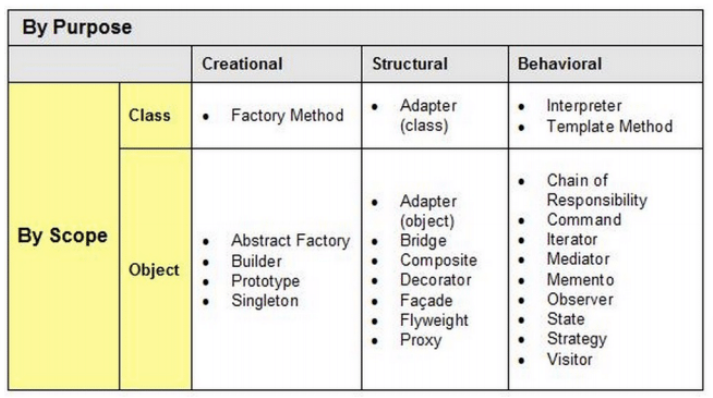
\includegraphics[scale=0.4]{Images/22.png}
\end{center}

Estes encontram-se fortemente ligados:

\begin{center}
    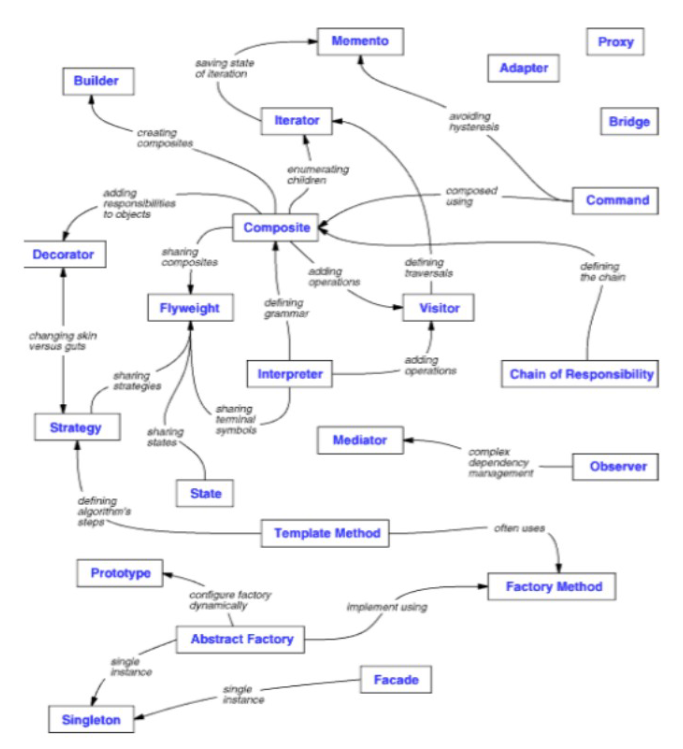
\includegraphics[scale=0.3]{Images/23.png}
\end{center}

\pagebreak

\begin{flushleft}
    \textbf{Nota:} Um bom programador deve, para além de conhecer conceitos de POO como herança, encapsulamento ou
    notação UML, de saber princípios OO, exemplos de bons desenhos e padrões de desenho!
\end{flushleft}


\section{Padrões Criacionais}

No que toca à construção de objetos, há dois grandes problemas:
O construtor de um objeto não pode devolver um subtipo do seu tipo (\textbf{Factory method}); 

\vspace{2mm}
O construtor devolve sempre uma nova instância daquela classe, não
permitindo a sua reutilização (\textbf{Singleton});

\subsection{Class: Factory Method}

\begin{flushleft}
    \textbf{Intenção -} O operador "new" é perigoso. Definir uma interface para criar
    um objeto numa superclasse, permitindo às subclasses alterar o tipo de objeto
    a ser criado, através de um construtor virtual.
\end{flushleft}

\begin{flushleft}
    \textbf{Problema -} É necessário estandardizar a arquitetura, continuando a permitir a aplicações
    individuais definir os seus objetos de domínio e permitir a sua instanciação.
\end{flushleft}

\begin{flushleft}
    \textbf{Solução -} Substituir as chamadas aos construtores de cada um dos objetos a criar, por
    chamadas ao método de fábrica (estático), passando um argumento que defina o
    tipo de objeto a construir, sendo devolvido um objeto deste tipo, também designado
    por produto.
\end{flushleft}

\begin{flushleft}
    \textbf{Estrutura:}

    \begin{center}
        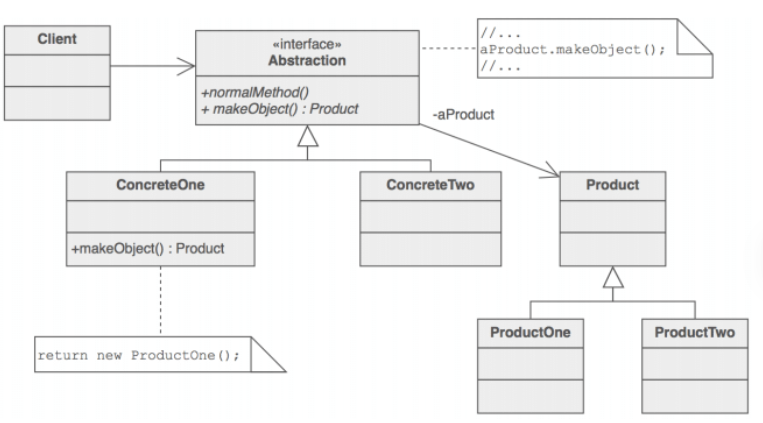
\includegraphics[scale=0.4]{Images/24.png}
    \end{center}
\end{flushleft}

\pagebreak

\begin{flushleft}
    \textbf{Check List:}

    \begin{enumerate}
        \item Se um construtor poder resultar em objetos inconsistentes, considerar
        desenhar um método fábrica;
        \item  Considerar fazer todos os construtores private ou protected;
        \item Se hierarquia tiver herança, considerar definir o método de fábrica na classe
        base;
        \item Considerar a criação de uma reserva de objetos criados (object pool), evitando assim a sua
        criação duplicada;
    \end{enumerate}


\end{flushleft}

\begin{flushleft}
    \textbf{Prós -} Permite que devolver uma instância de uma subclasse, a reutilização de um objeto já
    criado. Os métodos podem ter nomes mais sugestivos do que os construtores.

    É possível adicionar novos métodos de fábrica para novos produtos sem alterações
    para o cliente! 
\end{flushleft}

\begin{flushleft}
    \textbf{Exemplo:}

    \vspace{2mm}
    Num \textbf{Viveiro}, para criar uma \textbf{Árvore}, podemos ter um método de fábrica que aceite como argumento
    uma string e devolva um objeto do tipo \textbf{Árvore}, mas de uma subclasse. Assim, o programa principal fica
    liberto de fazer new, limitando-se a invocar o método estátido no \textbf{Viveiro}.

    \begin{center}
        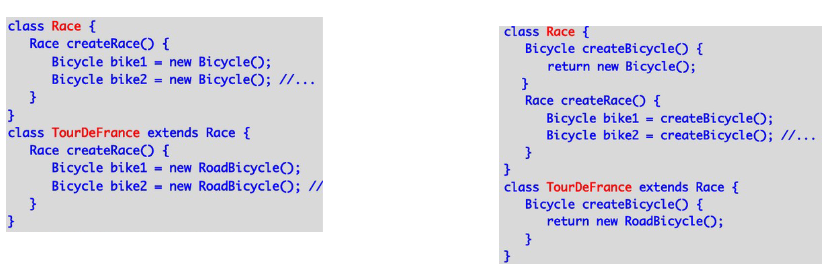
\includegraphics[scale=0.4]{Images/25.png}
    \end{center}

    \uline{Podem ser adicionadas novas corridas e bicicletas, sem modificações para o cliente.}

    \pagebreak

    Uma transportadora faz as suas entregas com carrinhas. No entanto, a determinada altura com o
    crescimento do volume de entregas e da sua abrangência geográfica começa a operar entregas em
    navios, o que não é suportado pelo seu programa.

    Para evitar este cenário e que o mesmo se repita cada vez que a transportadora começa a operar com um
    novo tipo de veículo, faz sentido utilizarmos o método de fábrica, definindo uma classe abstrata
    representante da \textbf{logística} e uma subclasse da mesma para cada tipo de veículo, devolvendo cada um
    um objeto deste tipo.

    \begin{center}
        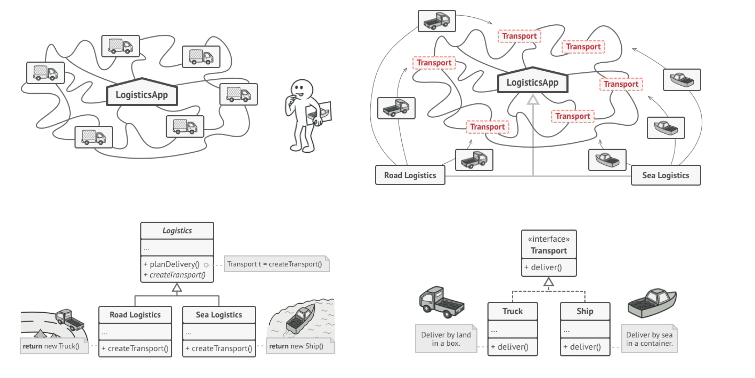
\includegraphics[scale=0.5]{Images/26.png}
    \end{center}
\end{flushleft}


\subsection{Object: Abstract Factory}

\begin{flushleft}
    \textbf{Intenção -} O operador "new" é perigoso. Criar uma interface para criar famílias de objetos relacionados sem especificar a sua
    classe, através de uma hierarquia que encapsula várias \textbf{plataformas} e a construção de
    vários \textbf{produtos}.
\end{flushleft}

\begin{flushleft}
    \textbf{Problema -} Devendo uma aplicação ser portátil, é necessário que encapsule as suas
    dependências.

    Estas plataformas podem ser: sistema de janelas, sistema operativo, base de dados\dots

    Este encapsulamento deve ser previsto no desenho do software.
\end{flushleft}

\begin{flushleft}
    \textbf{Solução -} Criar uma interface por produto, definindo para cada uma uma subclasse para cada
    plataforma e um método abstract factory com a interface e uma subclasse para
    cada plataforma, definindo um método para cada objeto, sendo o devolvido o
    correspondente a essa plataforma.
\end{flushleft}

\pagebreak

\begin{flushleft}
    \textbf{Estrutura:}

    \begin{center}
        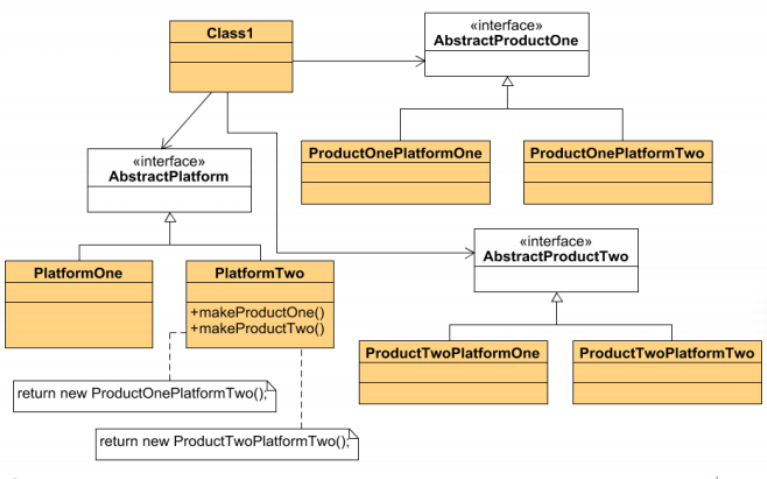
\includegraphics[scale=0.4]{Images/27.png}
    \end{center}
\end{flushleft}

\begin{flushleft}
    \textbf{Check List:}

    \begin{enumerate}
        \item Verificar se a independência da plataforma e a criação de serviços são um
        problema;
        \item  Planear a relação plataforma/produto;
        \item Definir uma interface fábrica para o método de fábrica por produto;
        \item Definir uma classe derivada para cada plataforma que encapsula todas as
        referências ao operador new;
        \item O cliente deve deixar de fazer referência ao operador "new", utilizando o
        método de fábrica para criar os produtos.
    \end{enumerate}
\end{flushleft}

\begin{flushleft}
    \textbf{Exemplo:}

    \begin{center}
        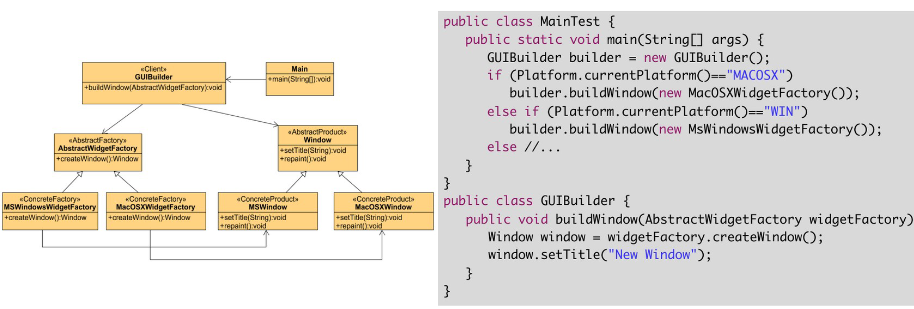
\includegraphics[scale=0.4]{Images/28.png}
    \end{center}

    \pagebreak

    \begin{center}
        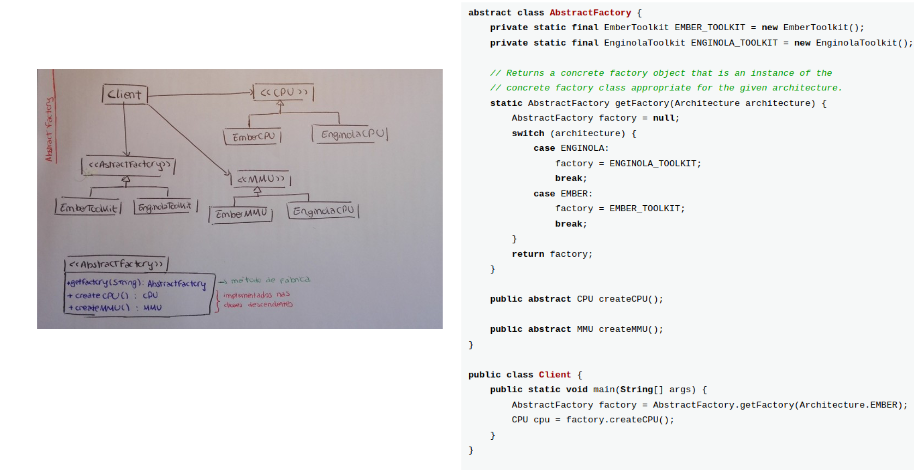
\includegraphics[scale=0.5]{Images/29.png}
    \end{center}

    \vspace{5mm}
    \begin{center}
        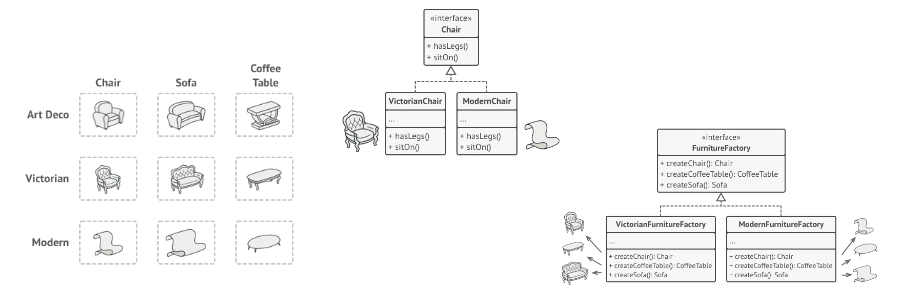
\includegraphics[scale=0.5]{Images/30.png}
    \end{center}
    
\end{flushleft}

\pagebreak

\subsection{Object: Builder}

\begin{flushleft}
    \textbf{Intenção -} Separar a construção de um objeto complexo da sua representação, de forma a que
    a construção (passo a passo) possa criar diferentes representações.

    Dando uma representação complexa, cria uma de muitas representações possíveis.
\end{flushleft}

\begin{flushleft}
    \textbf{Problema -} A construção de um objeto complexo geralmente implica um construtor com imensos
    parâmetros, alguns dos quais nem sempre necessitamos.
    
    Uma aplicação precisa de criar elementos de um agregado complexo. A
    especificação para o agregado existe num armazenamento secundário e uma de
    várias representações precisam de ser contruidas no armazenamento primário.

\end{flushleft}

\begin{flushleft}
    \textbf{Solução -} Retirar a criação do objeto da sua classe e movê-la para outra, o builder, um
    elemento secundário onde os vários elementos são armazenados para depois serem
    representados no primário (o objeto).

    Devemos assim de criar um abstract builder que é responsável por fazer os sets e
    um Director, responsável por gerir a construção do objeto.  
\end{flushleft}

\begin{flushleft}
    \textbf{Estrutura:}

    \begin{center}
        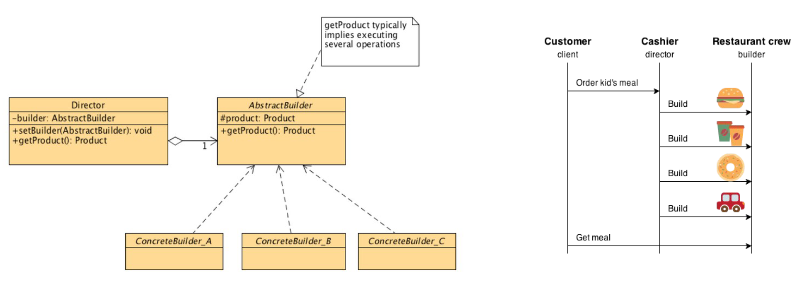
\includegraphics[scale=0.5]{Images/31.png}
    \end{center}

\uline{Ou, caso o objeto tenha muitos atributos, criar um builder inner class.}

\end{flushleft}


\begin{flushleft}
    \textbf{Nota:} Uma classe que utiliza este padrão é a StringBuilder. Sendo a classe String do tipo final, esta oferece uma
    alternativa à criação única dos objetos desse tipo, providenciando um armazenamento secundário e
    manipulável (com append()), devolvendo o objeto String construído aquando da invocação do método
    toString().
\end{flushleft}

\pagebreak

\begin{flushleft}
    \textbf{Check List:}

    \begin{enumerate}
        \item Verificar se o problema consiste em ter um input comum e vários outputs
        (representações) possíveis;
        \item Encapsular o input numa classe Director;
        \item Desenhar um protocolo para criar todas as representações possíveis (capturar os passos do protocolo num Builder interface);
        \item Definir uma classe derivada do builder para cada representação;
        \item O cliente cria um Director/Reader e um Builder, passando o último ao primeiro,
        pedindo de seguida ao Director que construa e devolva o produto;
        \item O cliente pede ao Director para "contruir";
        \item O cliente pede ao Builder para retornar o resultado;
    \end{enumerate}
\end{flushleft}

\begin{flushleft}
    \textbf{Exemplo:}

    \begin{center}
        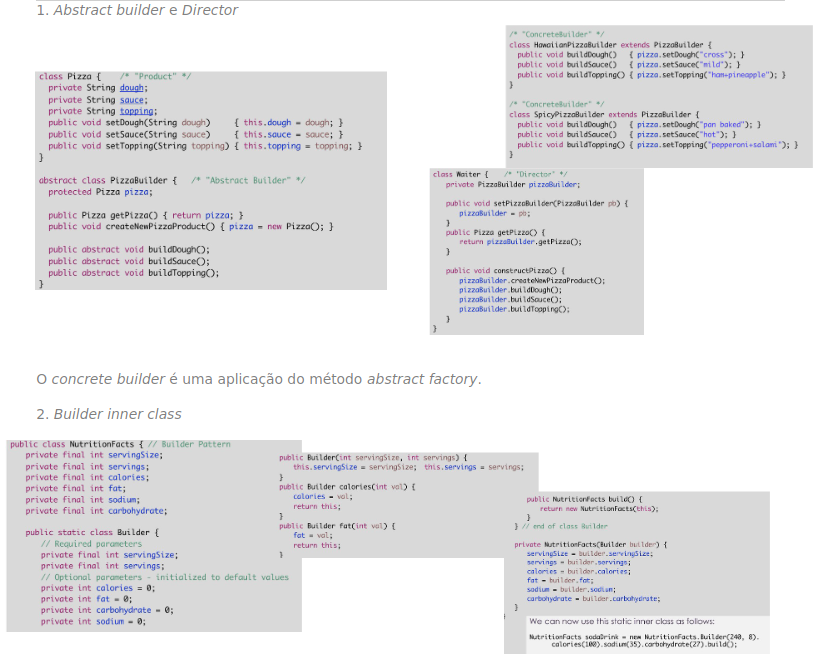
\includegraphics[scale=0.5]{Images/32.png}
    \end{center}

    \pagebreak

    \begin{center}
        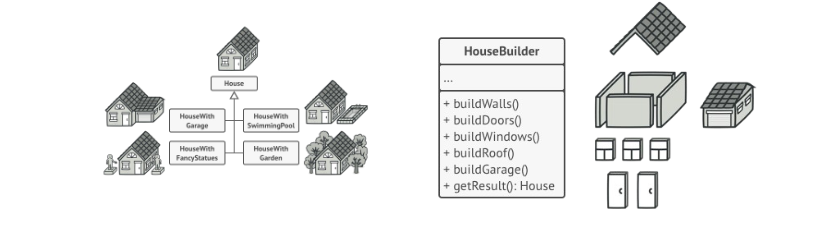
\includegraphics[scale=0.5]{Images/33.png}
    \end{center}
    
\end{flushleft}


\subsection{Object: Singleton}


\begin{flushleft}
    \textbf{Intenção -} Garantir que uma classe tem uma única instância e fornecer um ponto de acesso
    global à mesma.

    Encapsulação "just-in-time initialization" ou "initialization on first use".
\end{flushleft}

\begin{flushleft}
    \textbf{Problema -} É impossível de implementar com um construtor, uma vez que este cria uma nova
    instância do objeto por defeito. A criação de um ponto de acesso global também é
    um desafio, tal como a lazy initialization.

\end{flushleft}

\begin{flushleft}
    \textbf{Solução -} Definir o construtor como privado (private Singleton(String name)).

    Definir uma private static reference para um uńico objeto da classe (static private Singleton instance).

    Definir um método que vá buscar a instância (static public Singleton getInstance())
    (Os utilizadores apenas podem acessar o objeto Singleton através deste método)
\end{flushleft}

\begin{flushleft}
    \textbf{Estrutura:}

    \begin{center}
        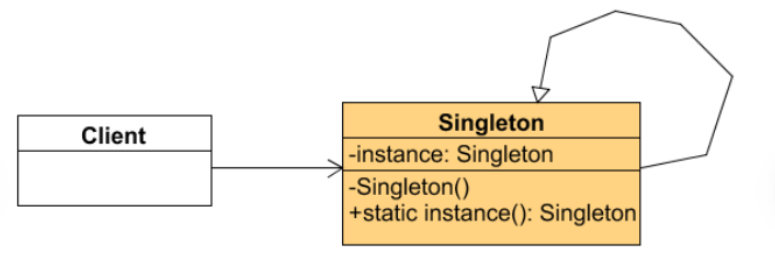
\includegraphics[scale=0.4]{Images/34.png}
    \end{center}

\end{flushleft}

\begin{flushleft}
    \textbf{Check List:}

    \begin{enumerate}
        \item Definir um atributo estático do seu tipo na classe;
        \item Definir um método público para lhe aceder. Com lazy initialization (criar se ainda não existe). Este deve ser o único método utilizado pelos clientes para lhe aceder.
        \item Definir todos os contrutores como protected ou private;
    \end{enumerate}
\end{flushleft}

\begin{flushleft}
    \textbf{Exemplo:} Um país só pode ter um governo. Mesmo que os elementos que o compõe mudem, em funções só existe
    uma instância do governo.
\end{flushleft}

\pagebreak

\subsection{Object: Object pool}

\begin{flushleft}
    \textbf{Intenção -} Aumentar a eficiência na utilização de objetos com custos elevados de inicialização,
    que são utilizados frequentemente, cuja instanciação simultânea é reduzida.

    Por exemplo conexões de rede/BD, threads...
\end{flushleft}

\begin{flushleft}
    \textbf{Problema -} Um cliente com acesso à Object Pool evita a criação de de novos objetos, basta pedir
    à Pool por um objeto que já foi previamente instanciado.
    
    É desejável manter todos os objetos disponíveis na mesma pool, de forma à sua
    reutilização ser feita de forma coerente.

\end{flushleft}

\begin{flushleft}
    \textbf{Solução -} Criar uma classe responsável por gerir os objetos reutilizáveis.
\end{flushleft}

\begin{flushleft}
    \textbf{Estrutura:}

    \begin{center}
        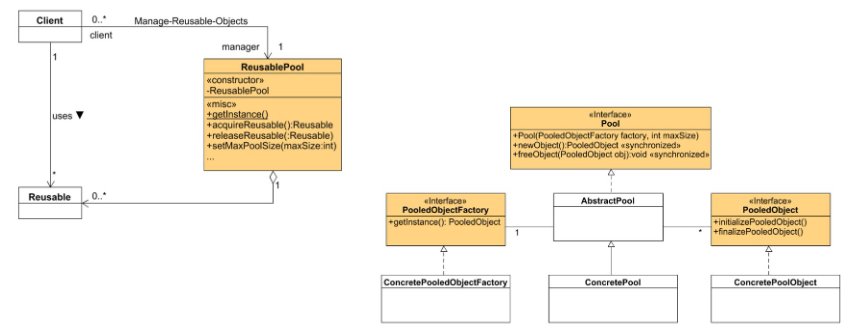
\includegraphics[scale=0.5]{Images/35.png}
    \end{center}

\end{flushleft}

\begin{flushleft}
    \textbf{Check List:}

    \begin{enumerate}
        \item Criar uma classe do tipo pool com uma coleção de pool objects;
        \item Criar métodos acquire() e release() nesta classe;
    \end{enumerate}
\end{flushleft}

\pagebreak

\begin{flushleft}
    \textbf{Exemplo:}

    \begin{center}
        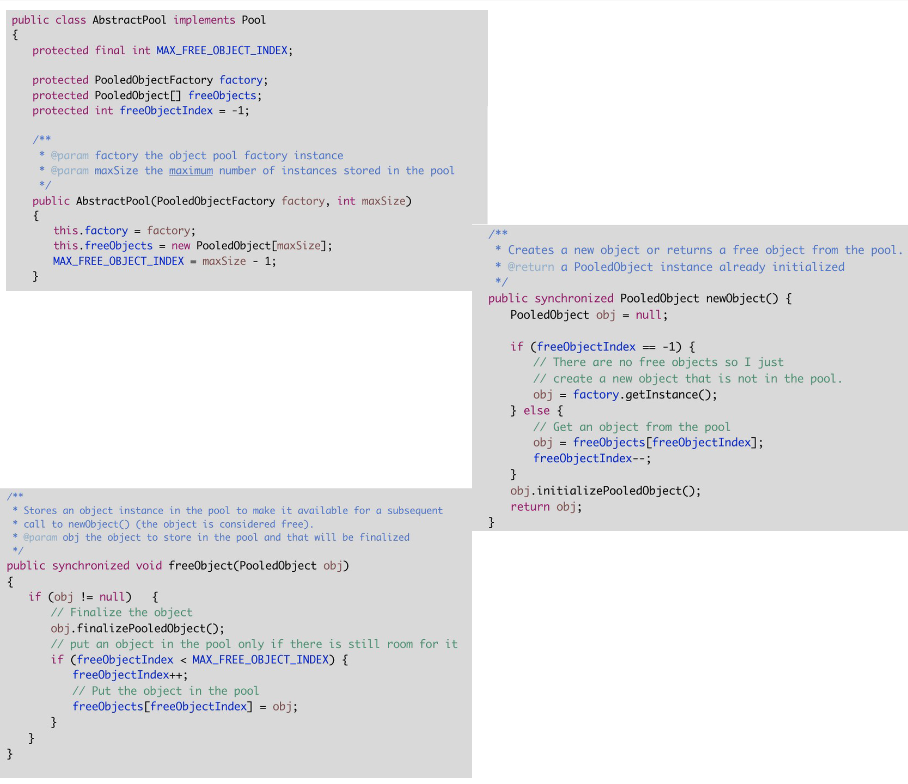
\includegraphics[scale=0.5]{Images/36.png}
    \end{center}
\end{flushleft}

\pagebreak

\subsection{Object: Prototype}

\begin{flushleft}
    \textbf{Intenção -} Criar objetos novos a partir de existentes, como protótipos, sem estar dependente
    das suas classes.

    O operador "new" é considerado perigoso.
\end{flushleft}

\begin{flushleft}
    \textbf{Problema -} A cópia de um objeto pressupõe a construção com os mesmos parâmetros e a
    definição dos restantes (não definidos no construtor) um a um. No entanto, por vezes
    há atributos privados a que não conseguimos aceder “de fora”.

\end{flushleft}

\begin{flushleft}
    \textbf{Solução -} Delegar o processo de clonagem no objeto a ser copiado, através de um método
    declarado numa interface comum a todos os objetos passíveis de clonagem.
\end{flushleft}

\begin{flushleft}
    \textbf{Estrutura:}

    \begin{center}
        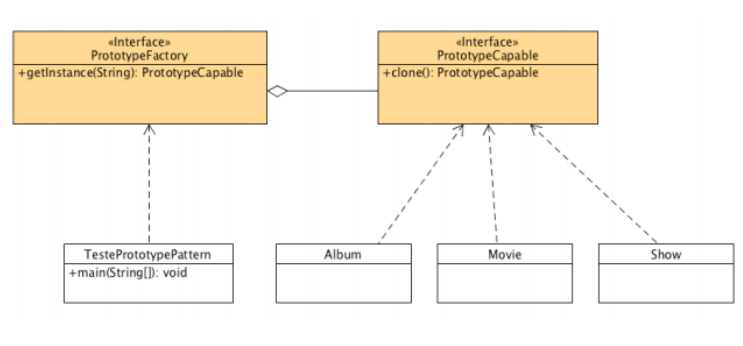
\includegraphics[scale=0.5]{Images/37.png}
    \end{center}

    Os objetos que implementam esta interface dizem-se \textbf{prototypes}.

    Os atributos privados podem ser copiados sem problema, uma vez que é possível um
    objeto aceder a um atributo privado de outro.

\end{flushleft}

\begin{flushleft}
    \textbf{Check List:}

    \begin{enumerate}
        \item Adicionar um método clone() ao produto;
        \item Desenhar um "registo" que mantém a cache dos objetos prototipáveis.
        
        Pode estar encapsulado numa classe do tipo factory, ou na classe base da
        hierarquia do produto.

        Pode ou não aceitar argumentos, descobre o protótipo correto a clonar e
        invoca o método clone(), retornando o seu resultado;

        \item O cliente substitui todas as referências ao operador "new" e substitui-las por
        invocações ao método de fábrica;
    \end{enumerate}
\end{flushleft}

\pagebreak

\begin{flushleft}
    \textbf{Exemplo:}

    \begin{center}
        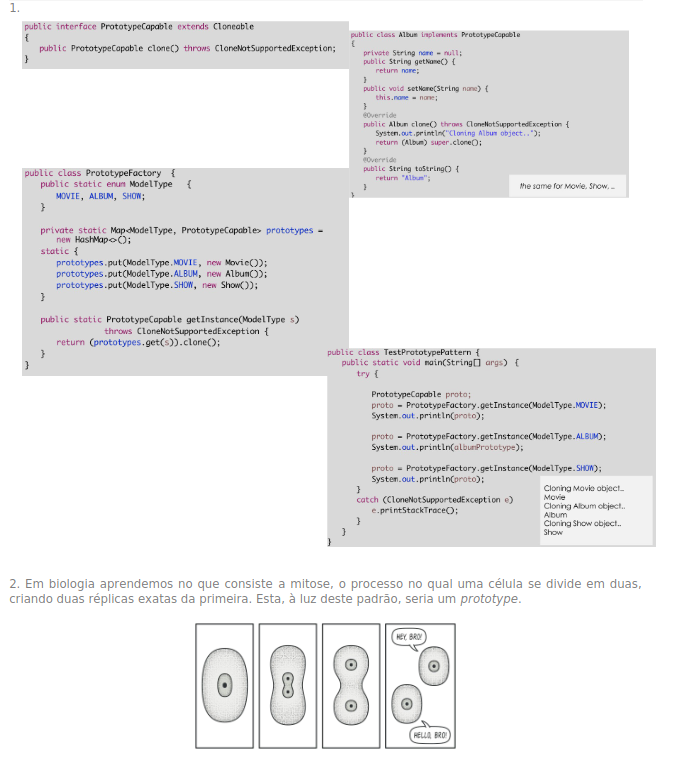
\includegraphics[scale=0.6]{Images/38.png}
    \end{center}
\end{flushleft}

\pagebreak

\subsection{Resumnindo}

\begin{flushleft}
    \textbf{Abstract Factory -} Cria uma instância de várias famílias de classes;

    \vspace{2mm}
    \textbf{Builder -} Separa a construção do objeto da sua representação;

    \vspace{2mm}
    \textbf{Factory Method -} Cria uma instância de várias classes derivadas;

    \vspace{2mm}
    \textbf{Singleton -} Uma classe da qual apenas exite uma única instância;

    \vspace{2mm}
    \textbf{Object Pool -} Evita a aquisição e libertação cara de requisitos através
    de objetos reciclados que já não estão em uso;

    \vspace{2mm}
    \textbf{Prototype -} Uma inicialização da instância completa para ser copiada ou clonada;


\end{flushleft}

\vspace{4mm}
\section{Padrões Estruturais}

Os padrões de desenho estruturais facilitam a construção de Software através da
identificação de formas simples de relacionar entidades.

\subsection{Class: Adapter}

\begin{flushleft}
    \textbf{Intenção -} Converter a interface de uma classe, de encontro aos requisitos do cliente. Permite
    assim a colaboração de objetos com interfaces incompatíveis, fornecendo uma nova
    interface a uma classe já existente.
\end{flushleft}

\begin{flushleft}
    \textbf{Problema -} Quando surge a necessidade de integrar um componente externo ao nosso
    ecossistema e este já existe, podemos reutilizá-lo. No entanto, por vezes surgem
    problemas de compatibilidade.

\end{flushleft}

\begin{flushleft}
    \textbf{Solução -} Nem sempre é desejável alterar código do componente que vamos reutilizar
    (trabalhosos e suscetível a erros e nem sempre temos a possibilidade de o
    manipular, pois pode ser uma ferramenta externa), sendo a solução a criação de um
    \textbf{adapter}, que é responsável por:

    \begin{enumerate}
        \item Fornecer uma interface, compatível com um dos objetos;
        \item Este objeto acede aos métodos desta interface;
        \item A cada chamada, o adapter passa o pedido ao segundo objeto, mas com a
        formatação adequada (processo de adaptação);
    \end{enumerate}

    O objeto “adaptado” não se apercebe da existência do adapter.
\end{flushleft}

\pagebreak

\begin{flushleft}
    \textbf{Estrutura:}

    \begin{center}
        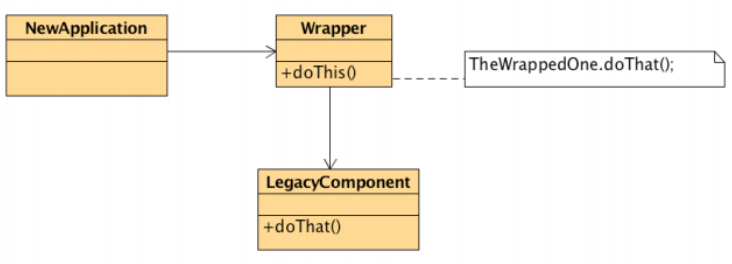
\includegraphics[scale=0.4]{Images/39.png}
    \end{center}

\end{flushleft}

\begin{flushleft}
    \textbf{Check List:}

    \begin{enumerate}
        \item Decide se a "independência da plataforma" e a serviços de criação são problemas;
        \item Escreve uma matriz "plataformas" versus "produtos";
        \item Define uma Interface fábrica que consiste num Factory Method por produto;
        \item Define uma classe derivada da fábrica para cada plataforma que encapsula
        todas as referências ao operador "new";
        \item O cliente não deve utilizar nenhum "new", e usar Factory Methods para criar os objetos de cada produto;
    \end{enumerate}
\end{flushleft}

\begin{flushleft}
    \textbf{Exemplo:} Uma analogia à vida real são as viagens internacionais, cenários em que muitas vezes nos deparamos com
    fichas diferentes das a que estamos habituados. A solução é utilizarmos um adaptador.

    No mundo tecnológico podemos pensar numa aplicação de monitorização das ações do mercado, que
    recorre a uma fonte de dados que os fornece em XML. Em determina altura surge a necessidade de
    integrar uma biblioteca de análise de dados, mas a que está disponível apenas faz o tratamento de dados
    JSON.

    Para a conseguirmos integrar sem fazer modificações neste componente, de forma simples e sem o
    modificar, podemos construir um adapter, acedido pelo componente, que consuta os dados na fonte em
    XML e os converte para JSON, passando depois esta informação ao novo componente (o cliente).

    \begin{center}
        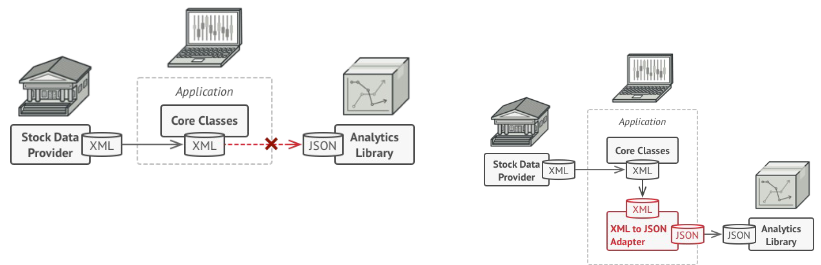
\includegraphics[scale=0.5]{Images/40.png}
    \end{center}
\end{flushleft}

\subsubsection{Subclassing vs Delegation}

Por vezes a adaptação não se trata de alterar o funcionamento dos métodos, mas de 
extender a classe a novos métodos, que fazem manipulação dos existentes.

Nesta situação temos duas abordagens distintas:

\vspace{3mm}
\textbf{Subclassing -} Acesso automático a todos os métodos da superclasse;

Mais eficiente;

\vspace{2mm}
\textbf{Delegation -} Permite a remoção de métodos;

Wrappers podem ser adicionados e removidos de forma dinâmica;

Composição múltipla de objetos;

Mais flexível;

\vspace{3mm}
\begin{flushleft}
    \textbf{Exemplo:}

    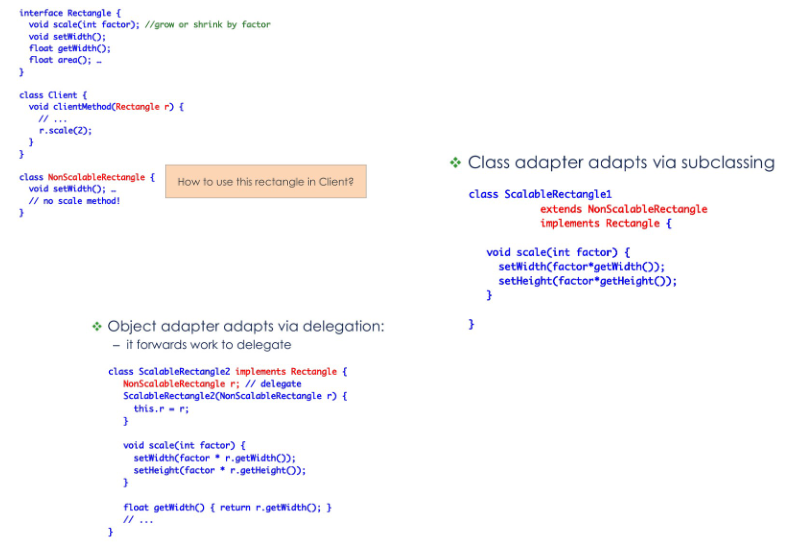
\includegraphics[scale=0.5]{Images/41.png}
\end{flushleft}

\pagebreak

\subsection{Object: Bridge}

\begin{flushleft}
    \textbf{Intenção -} Permitir a divisão de uma classe ou um conjunto de classes relacionadas em duas
    hierarquias: abstração e implementação, para que ambas possam ser desenvolvidas
    de forma independente.
\end{flushleft}

\begin{flushleft}
    \textbf{Problema -} Para criar implementações alternativas para uma classe uma
    hipótese é criar subclasses. No entanto, esta solução não é
    escalável, aumentando a sua complexidade exponencialmente
    com o número de variáveis envolvidas.

    \begin{center}
        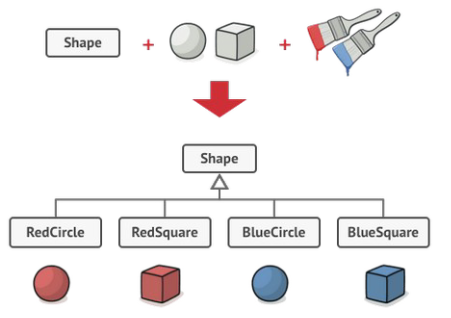
\includegraphics[scale=0.3]{Images/42.png}
    \end{center}

\end{flushleft}

\begin{flushleft}
    \textbf{Solução -} O problema prende-se com a extensão das classes em duas dimensões. A proposta
    deste padrão é deixar a herança e apostar na \uline{composição}, permitindo assim separar
    as dimensões em duas hierarquias de classes distintas.

    \begin{center}
        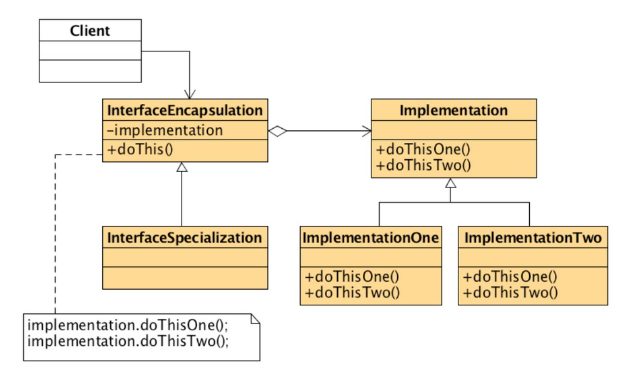
\includegraphics[scale=0.4]{Images/43.png}
    \end{center}
\end{flushleft}

\begin{flushleft}
    \textbf{Check List:}

    \vspace{3mm}
    Depois de verificar que existem duas dimensões variáveis no problema:
    \begin{enumerate}
        \item Desenhar a separação das mesmas, tendo em conta o que a plataforma
        fornece e os requisitos do cliente;
        \item Desenhar uma interface mínima, necessária e suficiente;
        \item Definir uma classe derivada dessa interface para cada plataforma;
        \item Criar uma \textbf{classe abstrata base}, que tem uma instância da plataforma, a
        que delega as suas funcionalidades;
        \item Definir \textbf{especializações} da classe abstrata, se necessário;
    \end{enumerate}
\end{flushleft}

\pagebreak

\begin{flushleft}
    \textbf{Exemplos:}

    \begin{center}
        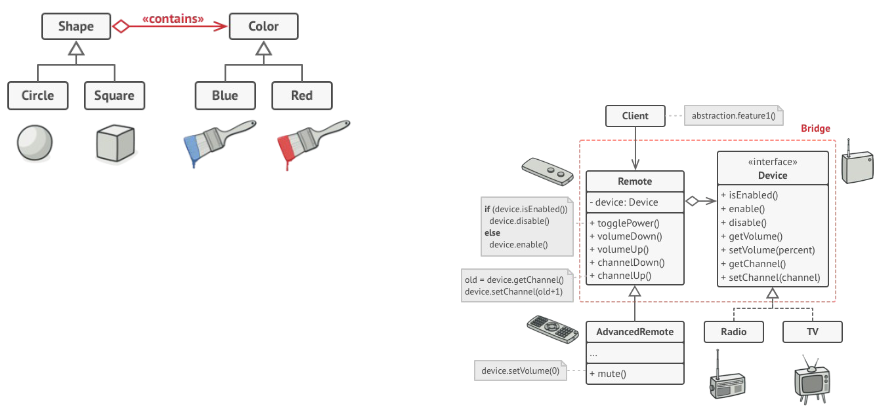
\includegraphics[scale=0.5]{Images/44.png}
    \end{center}
\end{flushleft}

\subsection{Object: Composite}

\begin{flushleft}
    \textbf{Intenção -} Ter componentes de produtos mas de forma a que um componente em si seja
    também um produto, ou seja, compor objetos em estruturas de árvore e utilizá-las
    como se fossem objetos (composição recursiva).

    "Diretórios possuem entradas, cada uma destas pode ser um diretório".

    1-to-many "has a" up the "is a" hierarchy.
\end{flushleft}

\begin{flushleft}
    \textbf{Problema -} Não é desejável que a aplicação tenha de distinguir um produto de uma composição
    de produtos.
\end{flushleft}

\begin{flushleft}
    \textbf{Solução -} Criar uma interface comum ao produto e à composição de produtos, sendo que esta
    última contém um atributo que é uma coleção de elementos desta interface.

    \begin{center}
        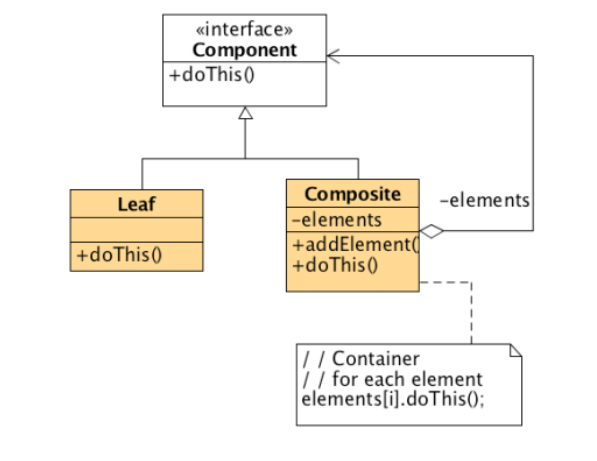
\includegraphics[scale=0.3]{Images/45.png}
    \end{center}
\end{flushleft}

\pagebreak

\begin{flushleft}
    \textbf{Check List:}

    \vspace{3mm}
    Se o problema for a representação de \uline{relações hierárquicas parte/todo}:
    \begin{enumerate}
        \item Considerar a heurística “caixas que contém produtos podem ser um produto
        em si”;
        \item Criar uma interface que torne os produtos e as caixas intercambiáveis,
        tanto o produto como a caixa estabelecem a relação is-a com a interface,
        a caixa estabelece a relação has-a com a interface one-to-many;
        \item Os métodos para adicionar e remover produtos da caixa devem ser
        declarados na classe da caixa (não na interface!);
    \end{enumerate}
\end{flushleft}

\begin{flushleft}
    \textbf{Exemplo:} Os sistemas de ficheiros são aplicações práticas e com as quais lidamos frequentemente deste padrão.
    Uma pasta (caixa) pode conter vários ficheiros (produtos), mas também outras pastas (novamente caixas)

    \begin{center}
        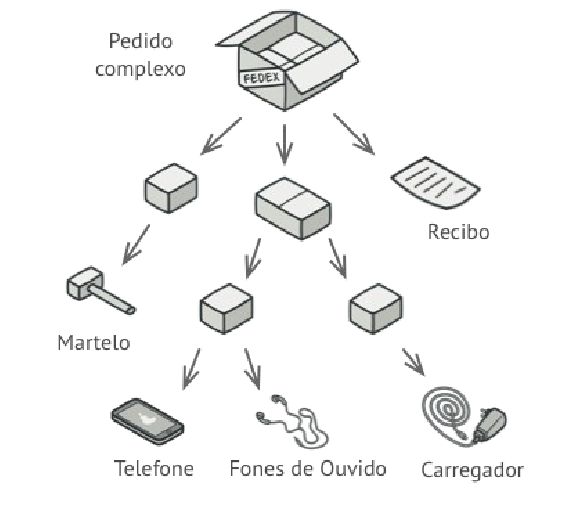
\includegraphics[scale=0.3]{Images/46.png}
    \end{center}
\end{flushleft}

\pagebreak

\subsection{Object: Decorator}

\begin{flushleft}
    \textbf{Intenção -} Adicionar novas responsabilidades a um objeto de forma dinâmica, colocando-lo
    “dentro” de outros objetos que têm esse comportamento.

    Client-specified embellishment of a core object by recursively wrapping it.

    Wrapping a gift, putting it in a box, and wrapping the box.
\end{flushleft}

\begin{flushleft}
    \textbf{Problema -} Para concretizar a intenção, uma opção é a herança. No entanto, se considerarmos
    várias funcionalidades que podem ser combinadas entre si (ou não), estaríamos a
    falar de demadiadas subclasses, pelo que esta não parece ser a solução adequada.
    
    Para além disto, a \uline{herança é estática}, não permitindo alterar o comportamento de
    um objeto em tempo de execução (a menos que substituído por um novo) e \uline{não há
    herança múltipla}, pelo que cada classe pode derivar de uma e de uma só.
\end{flushleft}

\begin{flushleft}
    \textbf{Solução -} A alternativa é a \textbf{agrageção ou composição}, criando num objeto (\textbf{wrapper})
    referência para outro, no qual delega alguma funcionalidade.

    O wrapper implementa o mesmo conjunto de métodos do alvo, no qual delega os
    pedidos que recebe, podendo, no entanto, manipular os dados antes ou depois de os
    passar.

    \begin{center}
        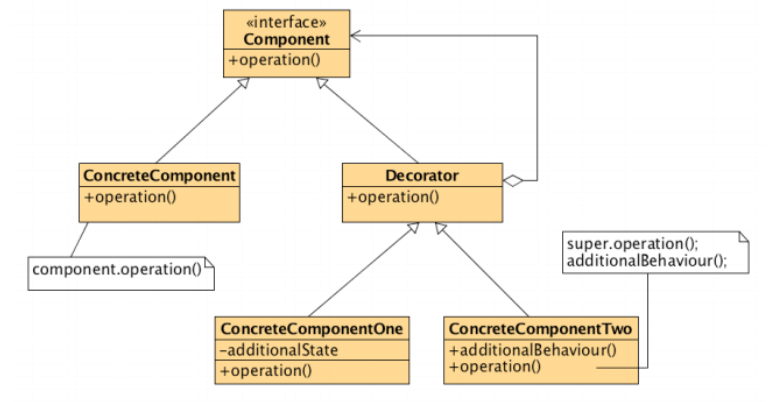
\includegraphics[scale=0.4]{Images/47.png}
    \end{center}
\end{flushleft}

\begin{flushleft}
    \textbf{Check List:}

    \vspace{3mm}
    Se estivermos perante um cenário com um \uline{componente central} e vários opcionais
    associados:
    \begin{enumerate}
        \item Criar uma interface que torne todas as classes intercambiáveis (estilo
        composite);
        \item Criar uma subclasse decorator, que suporte wrappers adicionais.
        
        Este têm como atributo um elemento da interface.
        
        Para cada componente opcional criar uma classe derivada;

        \item Tanto a classe do componente central como a decorator extendem a
        interface;
    \end{enumerate}
\end{flushleft}

\pagebreak

\begin{flushleft}
    \textbf{Exemplo:}

    \begin{center}
            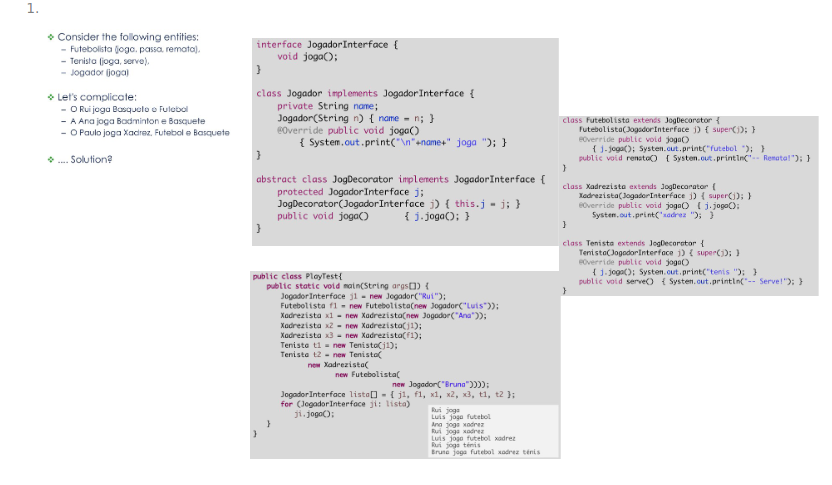
\includegraphics[scale=0.55]{Images/48.png}
    \end{center}

    \begin{center}
        \includegraphics[scale=0.4]{Images/49.png}
\end{center}
\end{flushleft}

\pagebreak

\subsection{Object: Façade}

\begin{flushleft}
    \textbf{Intenção -} Criar uma interface comum (e mais simples) a um conjunto (complexo) de interfaces
    num subsistema, facilitando a utilização do sistema.

    Envolver um subsistema complicado com uma interface simples.
\end{flushleft}

\begin{flushleft}
    \textbf{Problema -} Complexidade do sistema.
\end{flushleft}

\begin{flushleft}
    \textbf{Solução -} Implementar interface que utiliza apenas os métodos que o cliente necessita.

    \begin{center}
        \includegraphics[scale=0.35]{Images/50.png}
    \end{center}
\end{flushleft}

\begin{flushleft}
    \textbf{Check List:}

    \begin{enumerate}
        \item Identificar uma interface mais simples e unificada para o sistema
        (Só esta vai ser utilizada pelo cliente!);
        \item Desenhar um wrapper que encapsule todos os subsistemas.
        
        Responsável por delegar os métodos apropriados.
        
        Considerar se dentro dos subsistemas acrescentaria valor a criação de
        outras classes segundo o padrão façade;
    \end{enumerate}
\end{flushleft}

\begin{flushleft}
    \textbf{Beneficios:}

    \begin{enumerate}
        \item Ao esconder a implementação do cliente podemos alterar os subsistemas sem este
        se aperceber, promovendo um \uline{baixo acoplamento} e reduz as dependências.
        \item Não se pode dizer no entanto que adicione alguma funcionalidade ou que previna os
        clientes de aceder a determinados métodos.
    \end{enumerate}
\end{flushleft}

\pagebreak

\begin{flushleft}
    \textbf{Exemplos:}

    \begin{center}
        \includegraphics[scale=0.55]{Images/51.png}
    \end{center}
\end{flushleft}

\pagebreak

\subsection{Object: Flyweight}

\begin{flushleft}
    \textbf{Intenção -} Utilizar a partilha de forma a suportar muitos objetos compactos de forma eficiente.

    A estratégia Motif GUI, que substitui heavy-weight widgets por light-weight gadgets.
\end{flushleft}

\begin{flushleft}
    \textbf{Problema -} O desenho de objetos com baixos níveis de granularidade aumenta a flexibilidade,
    mas pode ter custos elevados no que toca à performance e utilização de memória
\end{flushleft}

\begin{flushleft}
    \textbf{Solução -} Separar os atributos comuns a todos os objetos dessa classe (estado intrínseco)
    dos específicos e mutáveis em cada um (estado extrínseco) em duas classes,
    sendo a que contém o estado extrínseco derivada da que tem o intrínseco.

    \begin{center}
        \includegraphics[scale=0.35]{Images/52.png}
    \end{center}

    Podemos ainda associar-lhes o padrão \uline{object pool}.
\end{flushleft}

\begin{flushleft}
    \textbf{Check List:}

    \vspace{3mm}
    Depois de verificar que uma grande quantidade de objetos de uma determinada
    classe estão a consumir demasiados recursos:

    \begin{enumerate}
        \item Identificar os atributos pertencentes ao estado intrínseco e extrínseco.
        
        Remover os extrínsecos e adicioná-los aos argumentos dos métodos que
        os utilizam;
        \item Criar uma fábrica segundo o padrão object pool.
        
        O cliente deve utilizar a fábrica em vez do operador new();
    \end{enumerate}
\end{flushleft}

\pagebreak

\begin{flushleft}
    \textbf{Exemplo:}

    \begin{center}
        \includegraphics[scale=0.5]{Images/53.png}
    \end{center}

    \vspace{1.5mm}
    \begin{center}
        \includegraphics[scale=0.45]{Images/54.png}
    \end{center}
\end{flushleft}

\pagebreak

\subsection{Object: Proxy}

\begin{flushleft}
    \textbf{Intenção -} Controlar o acesso ao objeto original, permitindo que se faça algo antes ou depois de
    chegar ao mesmo.

    Usar um nível extra de indirection para suportar acesso distríbuido, controlado ou inteligente.

    Adicionar um wrapper e uma delegation para proteger o componente verdadeiro da complexidade.
\end{flushleft}

\begin{flushleft}
    \textbf{Problema -} Lidar com objetos exigentes ao nível de recursos e sem a possibilidade de alterar o
    seu código (implementado o método object pool, p.e.) leva a que queiramos
    instanciá-los apenas quando e até serem necessários.
\end{flushleft}

\begin{flushleft}
    \textbf{Solução -} Criar uma classe \textbf{proxy} com a mesma interface do objeto original, que por sua vez
    passa tudo ao original, permitindo agora fazer algo antes ou depois da inicialização
    do mesmo.

    \begin{center}
        \includegraphics[scale=0.35]{Images/55.png}
    \end{center}

    Sendo invisível para o cliente, não vai afetar o seu código, ou seja, onde era
    esperado um objeto real pode ser colocado um proxy.
\end{flushleft}

\begin{flushleft}
    \textbf{Check List:}

    \begin{enumerate}
        \item Identificar a funcionalidade que a implementar no wrapper;
        \item Definir a interface que torne o proxy e o objeto real intercambiáveis;
        \item Considerar definir uma fábrica que decida qual dos dois é desejável;
        \item O proxy deve ter como atributo o objeto real;
    \end{enumerate}
\end{flushleft}

\pagebreak

\begin{flushleft}
    \textbf{Exemplo:}

    \begin{center}
        \includegraphics[scale=0.5]{Images/56.png}
    \end{center}

    \vspace{4mm}
    \begin{center}
        \includegraphics[scale=0.5]{Images/57.png}
    \end{center}
\end{flushleft}


\pagebreak

\section{Padrões de Comportamentais}

\subsection{Class: Chain of Responsibility}

\begin{flushleft}
    \textbf{Intenção -} Cria uma corrente de objetos que passam os pedidos através da mesma até que um deles o processe,
providenciando um único caminho para vários processamentos possíveis.
\end{flushleft}

\begin{flushleft}
    \textbf{Problema -} É necessário processar os pedidos de forma eficiente, sem mapeamento ou relações
de dependência.
\end{flushleft}

\begin{flushleft}
    \textbf{Solução -} Criar uma refência em cada handler para o seguinte, tendo cada um o poder de
passar ou não o pedido ao seguinte.
\end{flushleft}

\begin{center}
    \includegraphics[scale=0.3]{Images/58.png}
\end{center}

\begin{flushleft}
    \textbf{Check List:}

    \begin{enumerate}
        \item A classe base tem um ponteiro para o next;
        \item Cada classe derivada dá o seu contributo para o processamento do pedido;
        \item Caso o pedido deva ser passado ao handler seguinte, a classe derivada invoca
        a classe base para o fazer;
        \item O cliente cria e liga a corrente;
        \item O cliente “entrega” cada pedido na raiz da corrente;
    \end{enumerate}
\end{flushleft}

\begin{center}
    \includegraphics[scale=0.35]{Images/59.png}
\end{center}

\subsection{Class: Command}

\begin{flushleft}
    \textbf{Intenção -} Encapsular um pedido como num objeto, permitindo parameterizar métodos com
    diferentes pedidos, atrasar ou colocar a execução de um pedido numa fila e suportar
    operações que não podem ser feitas.
\end{flushleft}

\begin{flushleft}
    \textbf{Problema -} Necessitamos de fazer pedidos a objetos abstraíndo-nos sobre a operação a realizar
    e qual o recetor do pedido.
\end{flushleft}

\begin{flushleft}
    \textbf{Solução -} Dividir a aplicação em camadas, distinguindo a interface invocadora da
    implementação do processamento da invocação.
\end{flushleft}

\begin{center}
    \includegraphics[scale=0.35]{Images/60.png}
\end{center}

\begin{flushleft}
    \textbf{Check List:}

    \begin{enumerate}
        \item Se os pedidos tiverem de ser processados em vários momentos e/ou em diversas
        ordens.
    \end{enumerate}
\end{flushleft}

\begin{center}
    \includegraphics[scale=0.35]{Images/61.png}
\end{center}

\begin{center}
    \includegraphics[scale=0.35]{Images/62.png}
\end{center}

\subsection{Class: Iterator}

\begin{flushleft}
    \textbf{Intenção -} Percorrer objetos de uma coleção sem expor a sua representação (lista, árvore...).
\end{flushleft}    

\begin{flushleft}
    \textbf{Problema -} Em coleções mais complexas, podem haver várias formas de as percorrer. No
    entanto, implementá-las todas retira o foco da classe no armazenamento dos objetos
    (a sua principal utilidade).
\end{flushleft}

\begin{flushleft}
    \textbf{Solução -} Extrair o comportamento de travessia da coleção para outro objeto: um iterator.
\end{flushleft}
\vspace{4mm}
\begin{center}
    \includegraphics[scale=0.4]{Images/63.png}
\end{center}

\begin{flushleft}
    \textbf{Check List:}

    \begin{enumerate}
        \item Adicionar um método iterator() na classe da coleção, que devolva a classe do
        iterator;
        \item Desenhar a innerclass do iterator na classe agregadora;
        \item O cliente pede à classe agregadora para criar o iterator;
        O cliente utiliza os métodos hasNext() e next() para aceder aos elementos da
        coleção.
    \end{enumerate}
\end{flushleft}

\begin{center}
    \includegraphics[scale=0.35]{Images/64.png}
\end{center}

\begin{center}
    \includegraphics[scale=0.35]{Images/65.png}
\end{center}

\subsection{Class: Mediator}

\begin{flushleft}
    \textbf{Intenção -} Reduzir a dependência entre objetos, restringindo a comunicação direta, forçando
    que esta seja feita através de um mediador.
\end{flushleft}

\begin{flushleft}
    \textbf{Problema -} As dependências entre os objetos (pouca coesão) tornam-nos difíceis de reutilizar.
\end{flushleft}

\begin{flushleft}
    \textbf{Solução -} Colaboração indireta, através de um \textbf{mediador}.
\end{flushleft}

\begin{center}
    \includegraphics[scale=0.35]{Images/66.png}
\end{center}

O mediador define a interface que o Widget utiliza para comunicar, que por sua vez
define uma classe abstrata com referência ao mediador.
Do mediador pode descender um ConcreteMediator, que encapsula a lógica entre os
Widgets. Todos os descendentes do Widget comunicam exclusivamente através do
Intermediary.

\begin{flushleft}
    \textbf{Check List:}
    Se tivermos um conjunto de objetos que interagem entre si e beneficiariam do
    desacoplamento.
    \begin{enumerate}
        \item Encapsular as interações numa nova classe;
        \item Criar uma instância desta nova classe em todas as que interagiam;
        \item Equilibrar o desacoplamento com o princípio da distribuição equitativa de
        responsabilidades;
        \item Ter atenção para não criar um controlador ou objeto “deus”.
    \end{enumerate}
\end{flushleft}

\begin{center}
    \includegraphics[scale=0.35]{Images/67.png}
\end{center}

\subsection{Class: Memento}





\end{document}